% =============================================================================
%  Defensa TFG — Funciones de Base Hexaédricas de Nédélec en Julia
%  Presentación Beamer (tema JuanLesPins + color Crane)
%  Compilar con: pdflatex main.tex  (dos veces)
%
%  Las ecuaciones están extraídas de memoria/memoria_tfg.pdf y las imágenes de
%  memoria/imagenes/ y memoria/figuras/.
%
%  NOTAS SOBRE MULTIMEDIA
%  ----------------------
%  Este documento carga el paquete `multimedia`, que permite incrustar vídeos
%  con \movie[opciones]{poster}{archivo}. Los vídeos SOLO se reproducen en
%  visores PDF con soporte JavaScript (Adobe Acrobat / Acrobat Reader).
%  En visores como Okular, Evince o el visor de VS Code se mostrará únicamente
%  el póster (la imagen fija). Alternativa: paquete `media9` (\includemedia).
%  Los vídeos disponibles están en visualization/manim/media/videos/.
% =============================================================================
\documentclass{beamer}

\usetheme{JuanLesPins}
\usecolortheme{crane}

\usepackage[utf8]{inputenc}
\usepackage[T1]{fontenc}
\usepackage[spanish]{babel}
\usepackage{graphicx}
\usepackage{amsmath}
\usepackage{amssymb}
\usepackage{multimedia}
\usepackage{listings}
\usepackage{listingsutf8}
\usepackage{tikz}
\usetikzlibrary{positioning,shapes.geometric,shapes.misc,fit,backgrounds,calc,chains,arrows.meta}

% Definición del lenguaje Julia para listings (no viene de serie)
\lstdefinelanguage{Julia}{
  morekeywords={function,end,for,in,if,else,elseif,while,return,using,
    struct,mutable,module,import,export,let,begin,do,try,catch,const,
    true,false,nothing},
  sensitive=true,
  morecomment=[l]{\#},
  morecomment=[n]{\#=}{=\#},
  morestring=[b]",
  morestring=[b]',
}

% Mapeo de los caracteres griegos usados en el listado de Julia, para que
% listings (que no es UTF-8 nativo) los pueda imprimir correctamente.
\lstset{
  literate=%
    {ξ}{{$\xi$}}1
    {η}{{$\eta$}}1
    {ζ}{{$\zeta$}}1
}

% Estilo de los listados de código (comparación Julia / MATLAB / Fortran)
\lstset{
  basicstyle=\ttfamily\scriptsize,
  keywordstyle=\color{craneblue}\bfseries,
  commentstyle=\color{gray},
  stringstyle=\color{craneorange},
  showstringspaces=false,
  breaklines=true,
  columns=fullflexible,
  keepspaces=true,
  frame=single,
  framerule=0.3pt,
  rulecolor=\color{black!30},
  backgroundcolor=\color{black!3},
  xleftmargin=2pt,
  xrightmargin=2pt,
  aboveskip=2pt,
  belowskip=2pt
}

% Estilo de los listados de código Julia del paquete (uso del paquete y
% generación de coeficientes). Se define aquí, en el preámbulo, para poder
% usarlo en cualquier diapositiva.
\lstdefinestyle{codestyle}{%
  language=Julia,basicstyle=\ttfamily\scriptsize,
  keywordstyle=\color{craneblue}\bfseries,
  commentstyle=\color{craneorange}\itshape,
  escapeinside={(*}{*)},inputencoding=utf8}

% Estilos para el diagrama de flujo
\tikzset{
  etapa/.style={
    rectangle, rounded corners=2pt, draw=black!60, fill=blue!8,
    text width=1.85cm, align=center, minimum height=1.05cm,
    font=\scriptsize, inner sep=2pt
  },
  puente/.style={
    rectangle, rounded corners=2pt, draw=black!60, fill=orange!12,
    text width=2.4cm, align=center, minimum height=0.8cm,
    font=\scriptsize, inner sep=2pt
  },
  flujo/.style={-{Latex[length=1.6mm]}, draw=black!70, thick},
  etiq/.style={font=\tiny, inner sep=1pt}
}

% Ruta donde están las imágenes del repositorio (relativa a este archivo).
% La carpeta img/ contiene las versiones con fondo blanco de las figuras de
% Manim (originalmente renderizadas sobre fondo gris oscuro #2b2b2b).
\graphicspath{{img/}{../../memoria/imagenes/}{../../memoria/figuras/}{../../NedelecHex/output/}}

% ---------------------------------------------------------------------------
%  Macro auxiliar: figura pendiente de insertar (solo para las que faltan).
%  Uso: \figuraplaceholder{alto}{descripción}
% ---------------------------------------------------------------------------
\newcommand{\figuraplaceholder}[2]{%
  \begin{center}
    \fbox{\begin{minipage}[c][#1][c]{0.72\textwidth}
      \centering\itshape [Figura pendiente: #2]
    \end{minipage}}
  \end{center}
}

\title[]{Cálculo de Funciones de Base Hexaédricas de Elementos Finitos para Electromagnetismo en Julia}
\subtitle{Trabajo de Fin de Grado}
\author[Antonio García Marugán]{Antonio García Marugán}
\institute[UC3M]{Universidad Carlos III de Madrid}
\date{Octubre 2026}

% Pie de diapositiva: color uniforme, sin título del trabajo ni curso,
% con numeración de diapositiva a la derecha.
% JuanLesPins no trae footline por defecto, así que se define uno propio.
% Se usa el amarillo oscuro de la parte superior de la barra lateral
% (palette quaternary = craneorange) para que combine con la cabecera.
%
% NOTA sobre la numeración: se muestra «actual / total» donde el total es el
% número de diapositivas SIN contar los anexos. El total principal se guarda en
% el contador \mainframetotal justo antes de \appendix (donde \insertframenumber
% ya vale el número de diapositivas principales). Así el valor es correcto y
% estable en todas las pasadas de pdflatex, sin depender de \ref.
%
% En los anexos se reinicia el contador de diapositiva (\setcounter{framenumber}
% tras \appendix) y se activa el indicador \ifanexos, de modo que el pie muestra
% «actual / total» con el total de anexos (calculado como
% \inserttotalframenumber - \mainframetotal) en lugar del total principal.
% Portada de sección: en lugar del texto por defecto «Section N» (en inglés),
% se muestra el nombre de la sección en español.
\setbeamertemplate{section page}{%
  \centering
  \begin{beamercolorbox}[sep=12pt,center]{section title}
    \usebeamerfont{section title}\insertsection\par
  \end{beamercolorbox}
}

\newif\ifanexos
\anexosfalse
\setbeamercolor{pie}{bg=craneorange, fg=craneblue}
\setbeamertemplate{footline}{%
  \leavevmode%
  \hbox{%
    \begin{beamercolorbox}[wd=.4\paperwidth,ht=2.5ex,dp=1.125ex,center]{pie}%
      \usebeamerfont{author in head/foot}\insertshortauthor
    \end{beamercolorbox}%
    \begin{beamercolorbox}[wd=.4\paperwidth,ht=2.5ex,dp=1.125ex,center]{pie}%
      \usebeamerfont{date in head/foot}\insertshortdate
    \end{beamercolorbox}%
    \begin{beamercolorbox}[wd=.2\paperwidth,ht=2.5ex,dp=1.125ex,center]{pie}%
      \usebeamerfont{author in head/foot}%
      \ifanexos
        \insertframenumber\,/\,\ref{lastanexoframe}%
      \else
        \insertframenumber\,/\,\ref{lastmainframe}%
      \fi
    \end{beamercolorbox}%
  }%
  \vskip0pt%
}

\begin{document}

% ---------------------------------------------------------------------------
%  DIAPOSITIVA 1 — PORTADA
% ---------------------------------------------------------------------------
\begin{frame}
  \titlepage
\end{frame}

% ---------------------------------------------------------------------------
%  DIAPOSITIVA 2 — ÍNDICE
% ---------------------------------------------------------------------------
\begin{frame}{Índice}
  \tableofcontents
\end{frame}

% ===========================================================================
\section{Motivación y objetivos}
% ===========================================================================

% ---------------------------------------------------------------------------
%  DIAPOSITIVA 3 — Contexto de HOFEM
% ---------------------------------------------------------------------------
\begin{frame}{Contexto de HOFEM}
  \textbf{HOFEM} (\textit{Higher Order Finite Element Method}) del
  \textbf{GREMA} (UC3M).
  \begin{itemize}\setlength\itemsep{2pt}
    \item \textbf{Formulación débil} de la ecuación de onda vectorial de doble
      rotacional.
    \item Elementos \textbf{isoparamétricos curl-conformes de alto orden} de
      Nédélec.
    \item Implementados \textbf{tetraedros y prismas}, pero \textbf{no hexaedros}.
    \item Implementado en \textbf{Fortran}.
  \end{itemize}
\end{frame}

% ---------------------------------------------------------------------------
%  DIAPOSITIVA 5 — Lenguajes para prototipos vs. lenguajes para implementación
% ---------------------------------------------------------------------------
\begin{frame}[fragile]{Lenguajes para prototipos vs.\ lenguajes para implementación}
  \vspace{0.3cm}
  Evaluación de $\xi\eta^2\zeta^2$ y medida del tiempo que tardan:
  \vspace{0.1cm}

  \begin{columns}[t]
    \begin{column}{0.36\textwidth}
      \textbf{\color{craneblue}Fortran}
      \begin{lstlisting}[language=Fortran,basicstyle=\ttfamily\fontsize{5.5}{6}\selectfont]
program sumsq
  implicit none
  integer, parameter :: n = 200
  integer :: i, j, k
  real(8) :: xi, eta, zeta, total
  real(8) :: t0, t1
  call cpu_time(t0)
  total = 0.0d0
  do i = 1, n
    xi = dble(i)/n
    do j = 1, n
      eta = dble(j)/n
      do k = 1, n
        zeta = dble(k)/n
        total = total + xi*eta**2*zeta**2
      end do
    end do
  end do
  call cpu_time(t1)
end program sumsq
\end{lstlisting}
      \vspace{0.05cm}
      \centering\textbf{8{,}6\,ms}
    \end{column}
    \begin{column}{0.30\textwidth}
      \textbf{\color{craneblue}MATLAB}
      \begin{lstlisting}[language=Matlab,basicstyle=\ttfamily\fontsize{5.5}{6}\selectfont]
n = 200;
tic;
total = 0.0;
for i = 1:n
  xi = i/n;
  for j = 1:n
    eta = j/n;
    for k = 1:n
      zeta = k/n;
      total = total + xi*eta^2*zeta^2;
    end
  end
end
t = toc;
\end{lstlisting}
      \vspace{0.05cm}
      \centering\textbf{6\,900\,ms}
    \end{column}
    \begin{column}{0.30\textwidth}
      \textbf{\color{craneblue}Julia}
      \begin{lstlisting}[language=Julia,basicstyle=\ttfamily\fontsize{5.5}{6}\selectfont]
n = 200
total = 0.0
t = @elapsed begin
  for i in 1:n
    ξ = i/n
    for j in 1:n
      η = j/n
      for k in 1:n
        ζ = k/n
        total += ξ*η^2*ζ^2
      end
    end
  end
end
\end{lstlisting}
      \vspace{0.05cm}
      \centering\textbf{13{,}3\,ms}
    \end{column}
  \end{columns}
\end{frame}

% ---------------------------------------------------------------------------
%  DIAPOSITIVA 6 — ¿Por qué hexaedros?
% ---------------------------------------------------------------------------
\begin{frame}{¿Por qué hexaedros?}
  \begin{columns}[t]
    \begin{column}{0.34\textwidth}
      \centering
      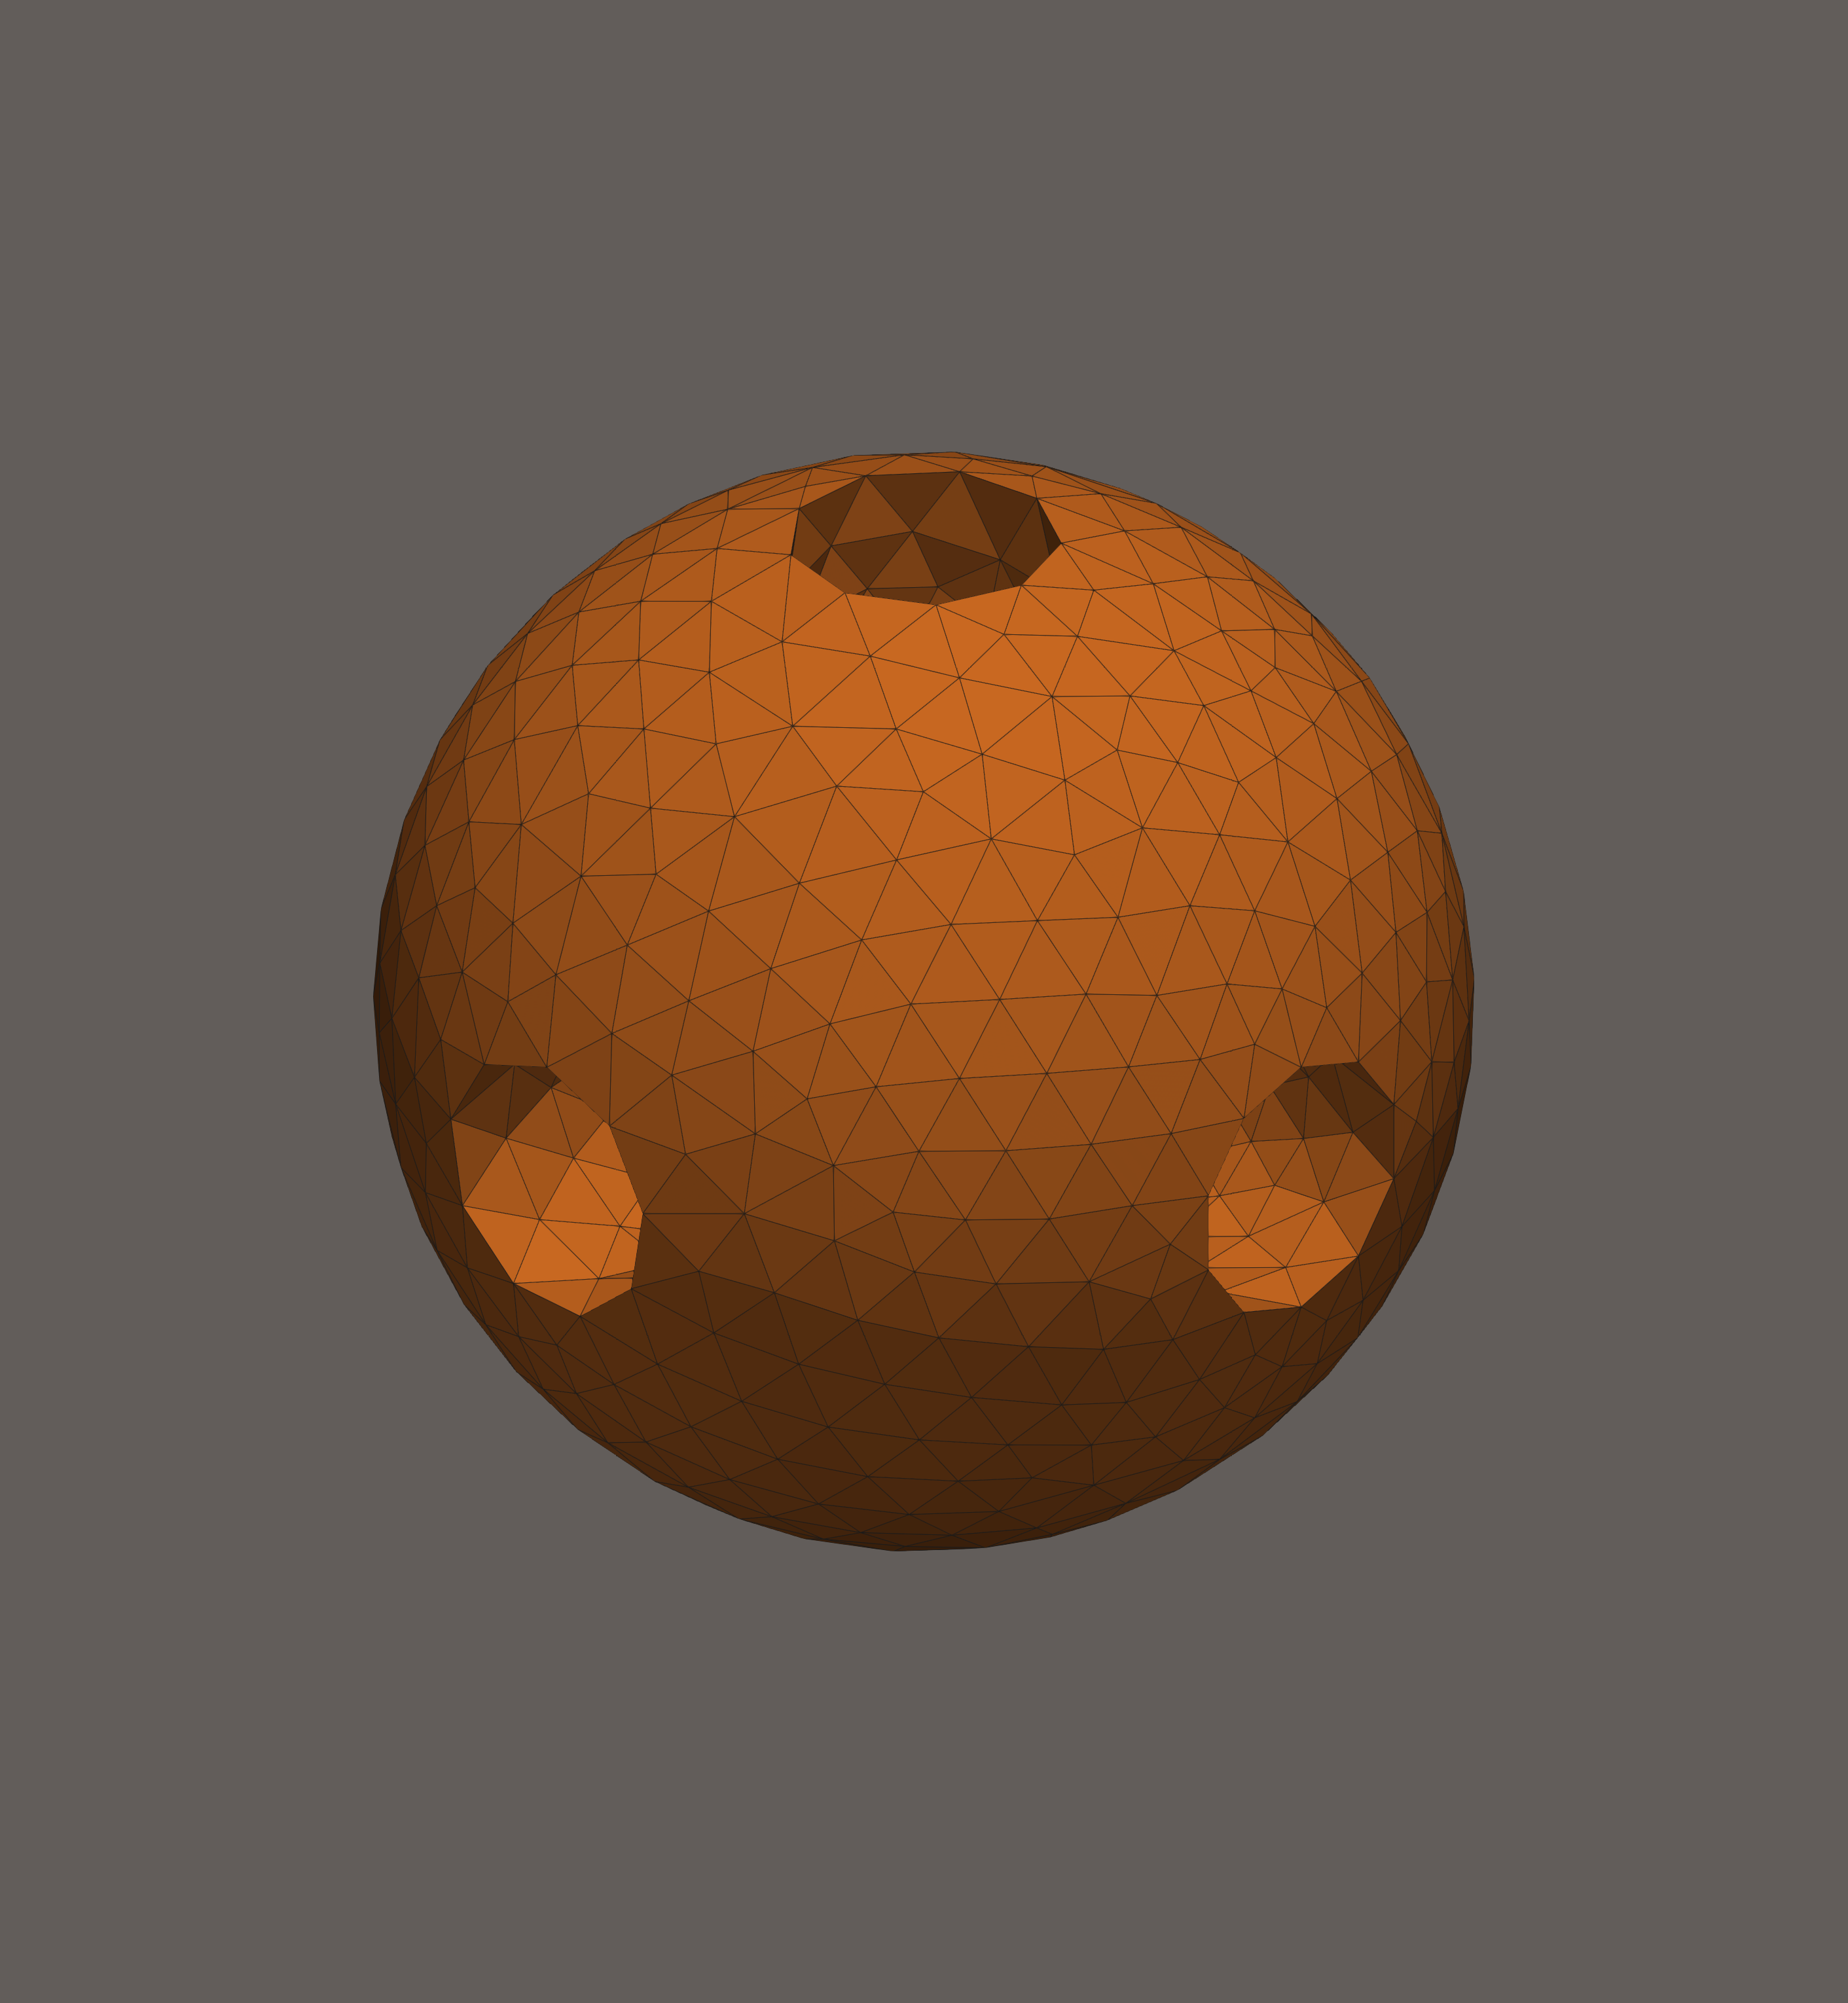
\includegraphics[width=0.92\textwidth]{malla_tetra.png}\\[2pt]
      \textbf{Tetraedros}\\[2pt]
      {\scriptsize
        \textcolor{green!60!black}{\textbf{+}} Mayor versatilidad
        geométrica\\[1pt]
        \textcolor{red!70!black}{\textbf{--}} Más elementos para la misma
        precisión}
    \end{column}
    \begin{column}{0.34\textwidth}
      \centering
      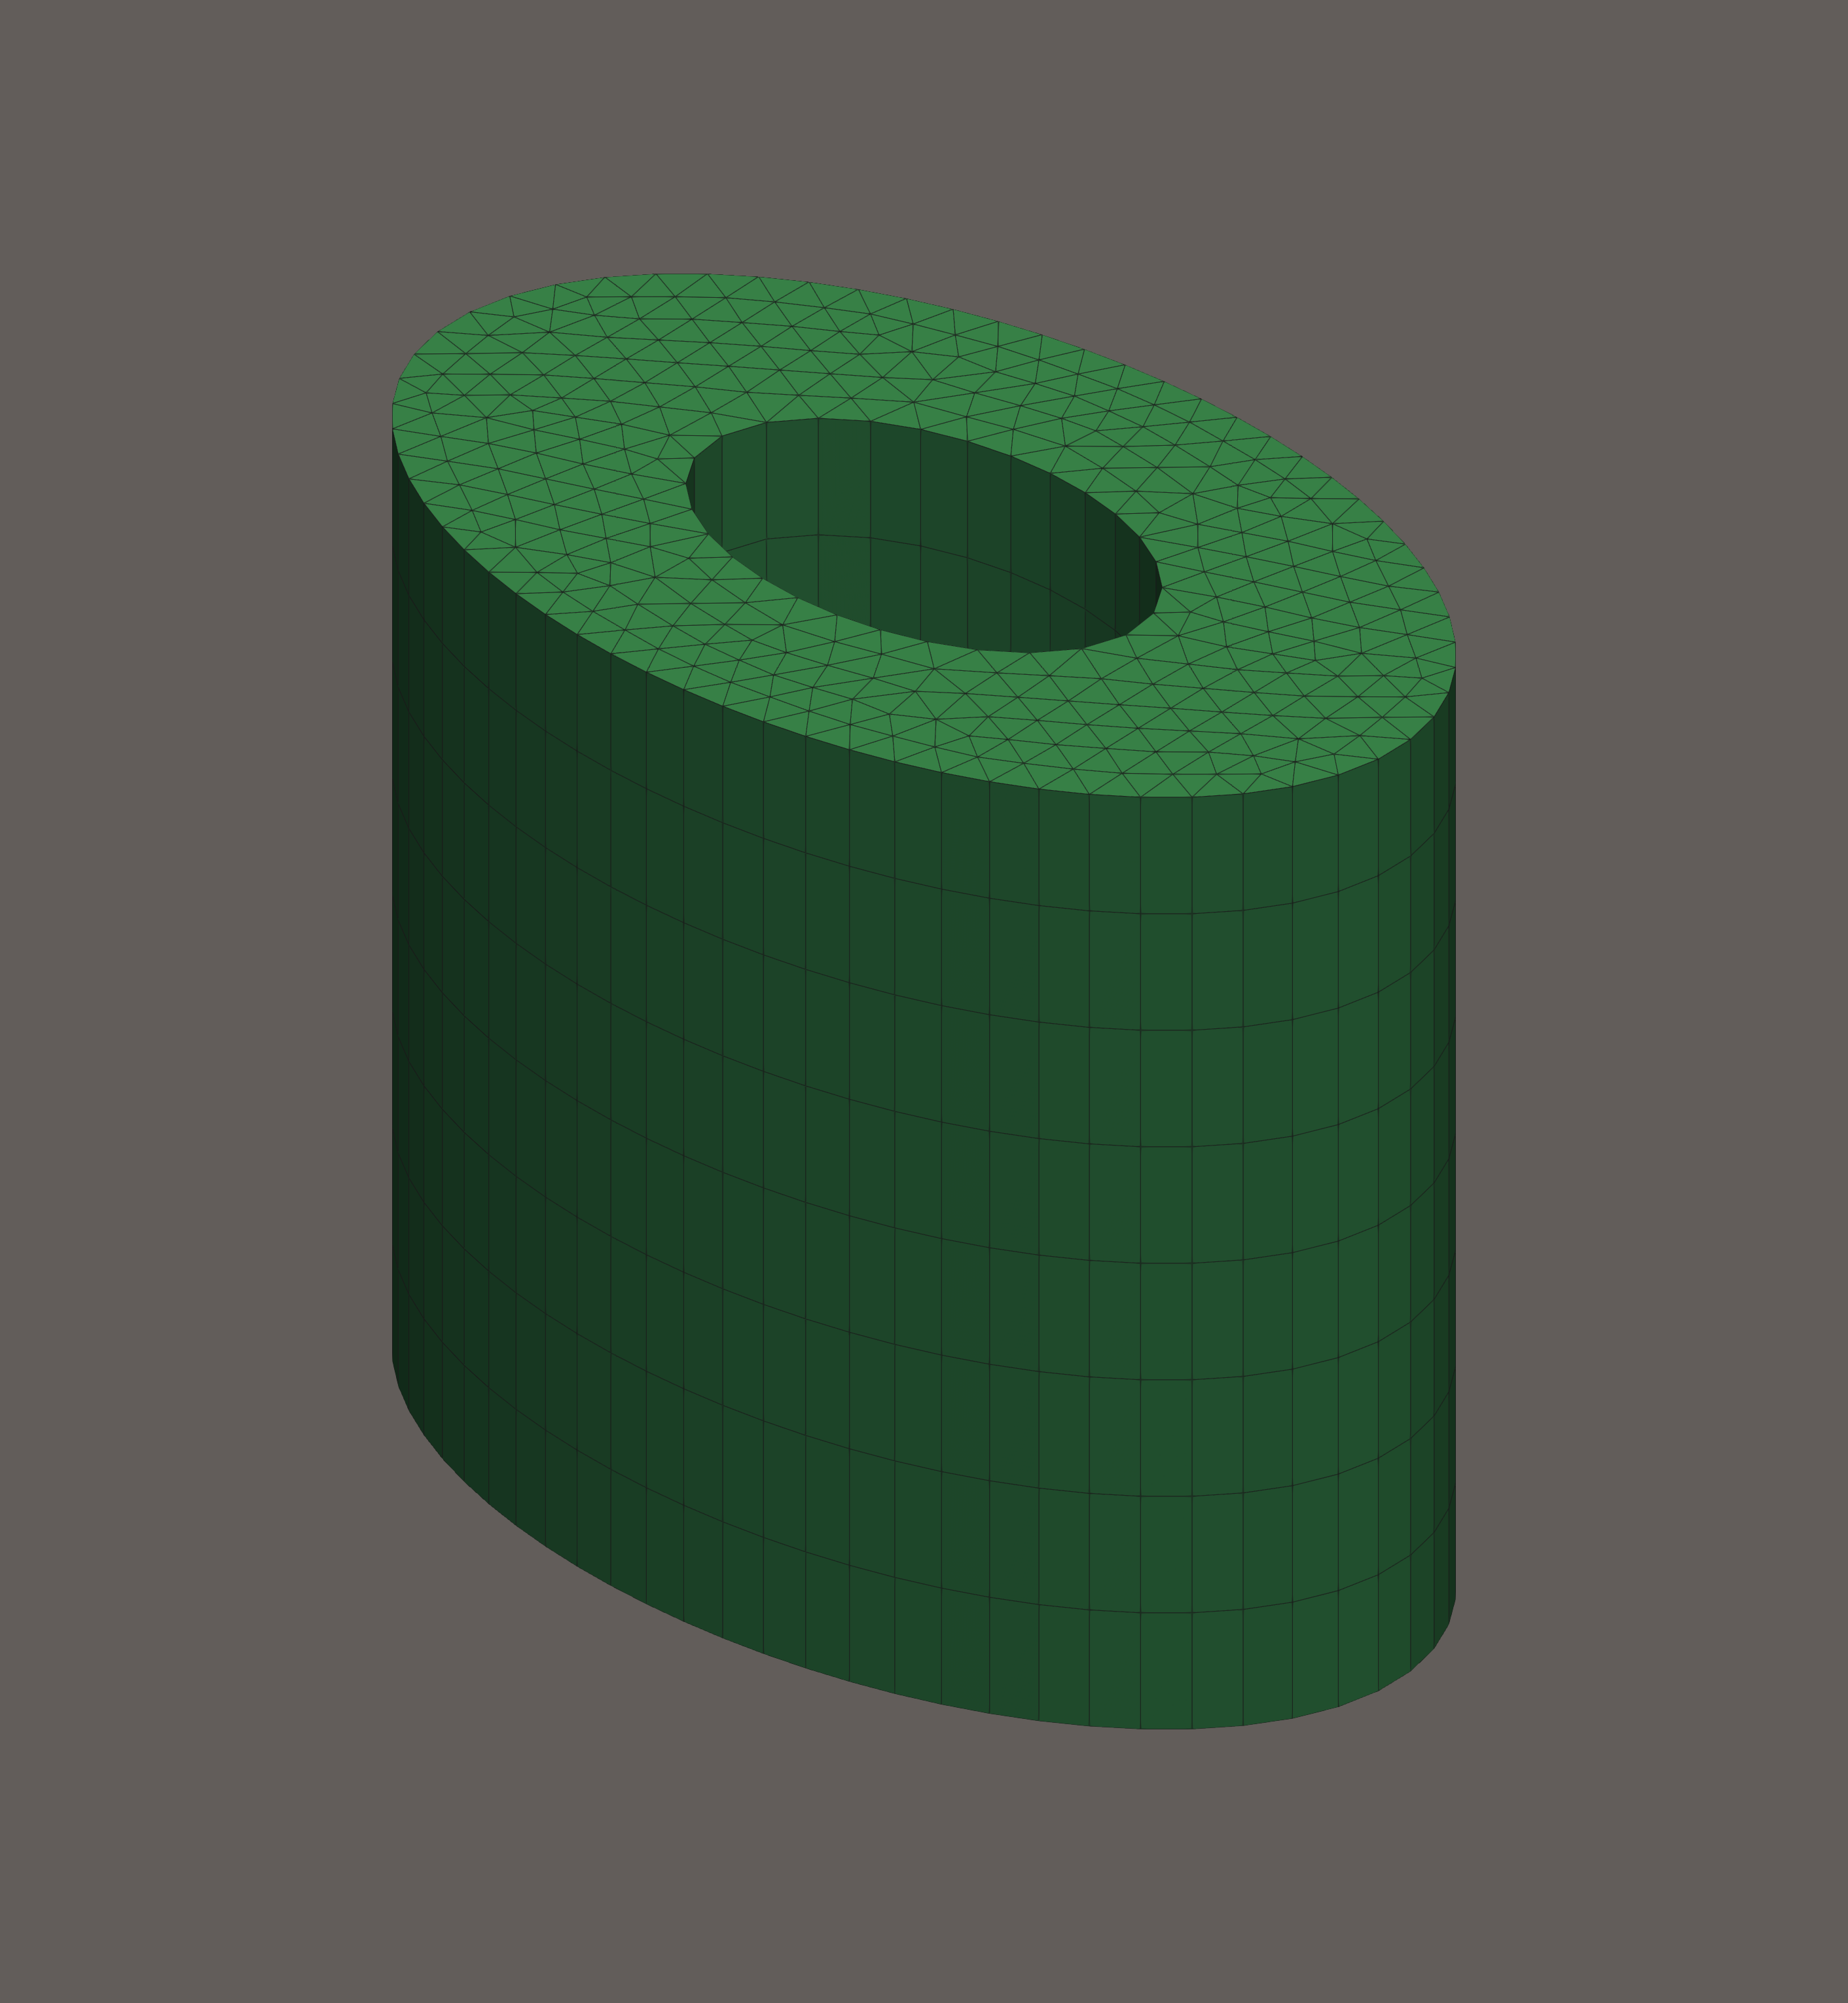
\includegraphics[width=0.92\textwidth]{malla_prismas.png}\\[2pt]
      \textbf{Prismas}\\[2pt]
      {\scriptsize
        \textcolor{green!60!black}{\textbf{+}} Ideal para extrusión y
        geometrías deformadas\\[1pt]
        \textcolor{red!70!black}{\textbf{--}} Menos flexibles que los
        tetraedros}
    \end{column}
    \begin{column}{0.34\textwidth}
      \centering
      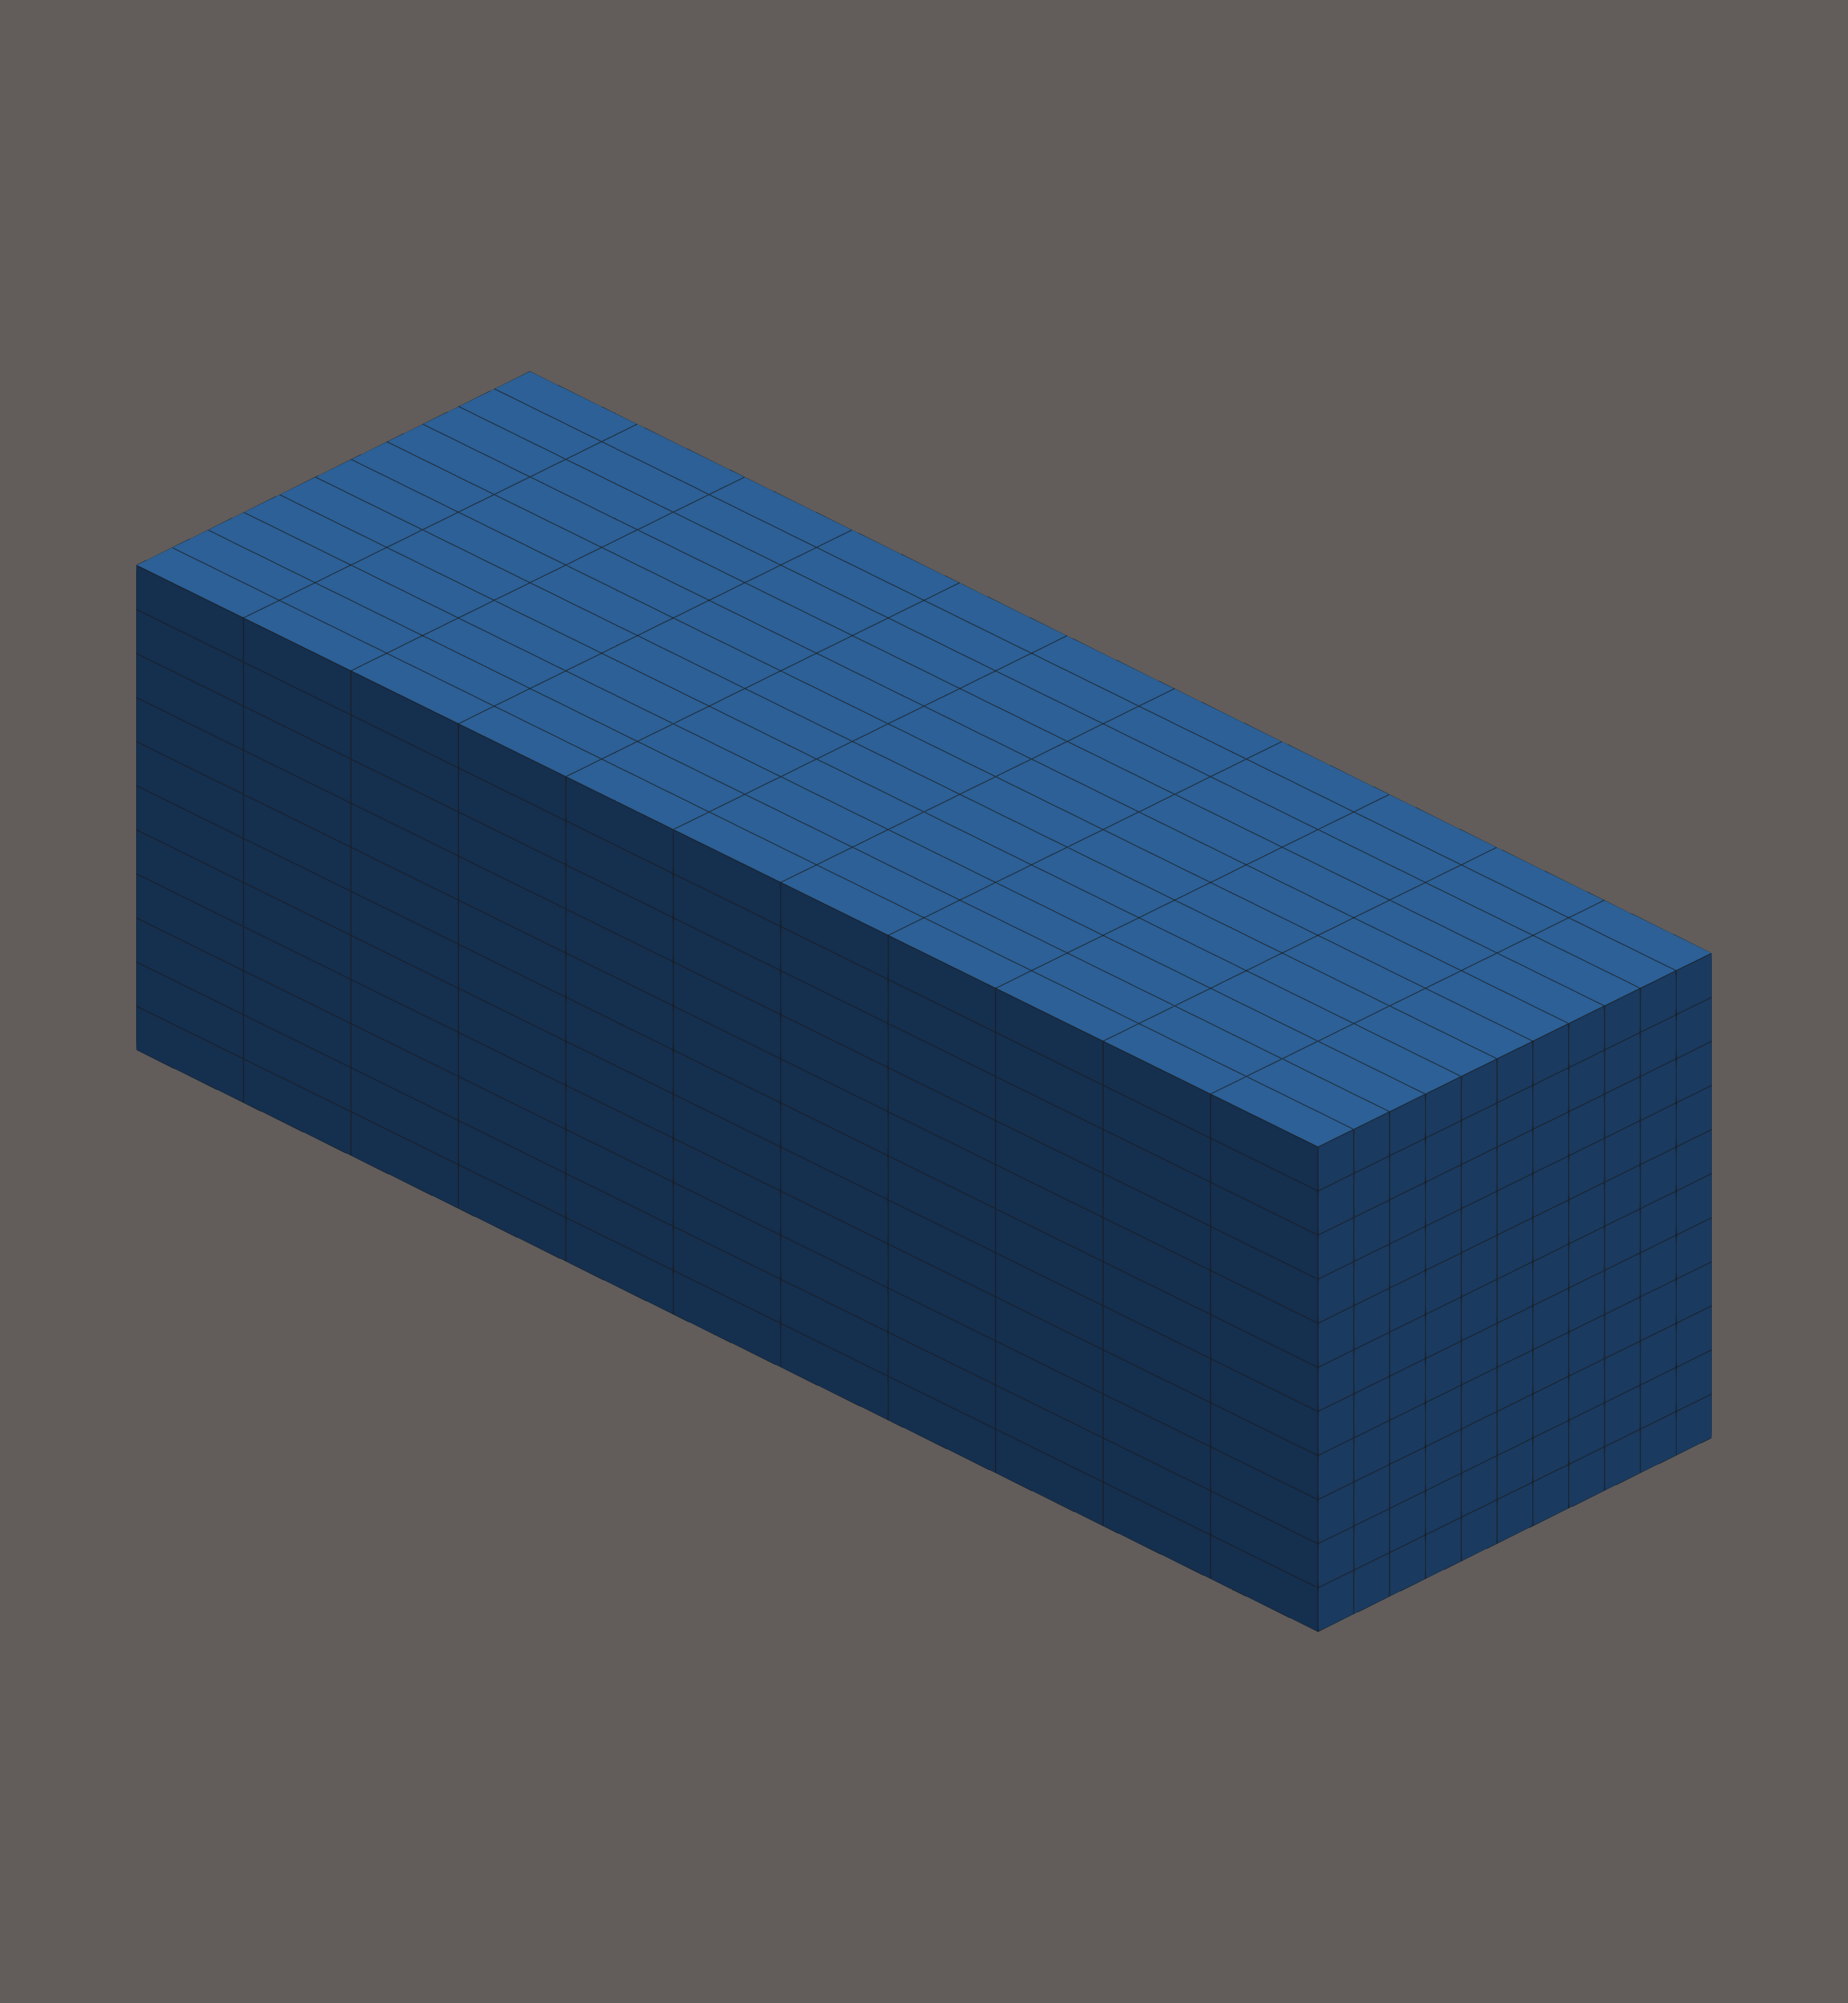
\includegraphics[width=0.92\textwidth]{malla_hexa.png}\\[2pt]
      \textbf{Hexaedros}\\[2pt]
      {\scriptsize
        \textcolor{green!60!black}{\textbf{+}} En estructuras regulares:
        \textbf{menos DOF} y mejor número de acondicionamiento\\[1pt]
        \textcolor{red!70!black}{\textbf{--}} Menos versátiles
        geométricamente}
    \end{column}
  \end{columns}
\end{frame}

% ---------------------------------------------------------------------------
%  DIAPOSITIVA 7 — Objetivos principales
% ---------------------------------------------------------------------------
\begin{frame}{Objetivos principales}
  \begin{itemize}
    \item \textbf{O1.} Implementar las funciones de base y los módulos para evaluarlas
    \item \textbf{O2.} Obtener los coeficientes y reproducir la Tabla II del artículo
    \item \textbf{O3.} Verificar el ensamblaje global: comprobar la dimensión del
      núcleo de $K$ y comparar las matrices $K$ y $M$ con MATLAB
    \item \textbf{O4.} Reproducir el benchmark de la cavidad semillena y su convergencia
    \item \textbf{O5.} Comparar el rendimiento frente a MATLAB
  \end{itemize}
\end{frame}

% ===========================================================================
\section{Fundamentos teóricos}
% ===========================================================================

% ---------------------------------------------------------------------------
%  DIAPOSITIVA 8 — Portada de sección
% ---------------------------------------------------------------------------
\begin{frame}
  \sectionpage
\end{frame}

% ---------------------------------------------------------------------------
%  DIAPOSITIVA 9 — Ecuaciones de Maxwell
% ---------------------------------------------------------------------------
\begin{frame}{Ecuaciones de Maxwell}
  Para un medio lineal e isótropo, en el dominio de la frecuencia (forma fasorial):
  \begin{center}
  \begin{minipage}{0.86\textwidth}
    \begin{block}{Ecuaciones de Maxwell en forma fasorial}
      \centering
      $\displaystyle
      \begin{aligned}
        \nabla \times \mathbf{E} &= -j\omega\mu\mathbf{H}
          && \text{(Faraday)} \\
        \nabla \times \mathbf{H} &= j\omega\varepsilon\mathbf{E} + \mathbf{J}
          && \text{(Ampère--Maxwell)} \\
        \nabla \cdot (\varepsilon\mathbf{E}) &= \rho
          && \text{(Gauss)} \\
        \nabla \cdot (\mu\mathbf{H}) &= 0
          && \text{(Gauss magnética)} \\
        \nabla \cdot \mathbf{J} &= -j\omega\rho
          && \text{(continuidad)}
      \end{aligned}$
    \end{block}
  \end{minipage}
  \end{center}
\end{frame}

% ---------------------------------------------------------------------------
%  DIAPOSITIVA 10 — Ecuación de onda
% ---------------------------------------------------------------------------
\begin{frame}{Ecuación de onda de Helmholtz}
  \vspace{-0.25cm}
  \setlength{\abovedisplayskip}{2pt}
  \setlength{\belowdisplayskip}{2pt}
  \begin{center}
  \begin{minipage}{0.94\textwidth}
    \small
    \textbf{1.} Maxwell \textbf{sin fuentes} ($\mathbf{J}=\mathbf{0}$, $\rho=0$):
    \[
      \nabla\times\mathbf{E} = -j\omega\mu_0\mu_r\mathbf{H},
      \qquad
      \nabla\times\mathbf{H} = j\omega\varepsilon_0\varepsilon_r\mathbf{E}.
    \]
    \textbf{2.} Aplicamos el rotacional a la ley de Faraday y sustituimos
    $\nabla\times\mathbf{H}$ de Ampère--Maxwell:
    \[
      \nabla\times(\nabla\times\mathbf{E})
      = -j\omega\mu_0\mu_r\,(\nabla\times\mathbf{H})
      = \omega^2\mu_0\varepsilon_0\,\mu_r\varepsilon_r\,\mathbf{E}.
    \]
    \textbf{3.} Dividimos entre $\mu_r$ y usamos $k_0^2=\omega^2\mu_0\varepsilon_0$:
    \begin{block}{Ecuación de onda de Helmholtz}
      \centering
      $\displaystyle
        \nabla \times \left( \frac{1}{\mu_r} \nabla \times \mathbf{E} \right)
        - k_0^2\, \varepsilon_r\, \mathbf{E} = \mathbf{0}
        \qquad \text{en } \Omega$
    \end{block}
  \end{minipage}
  \end{center}
\end{frame}

% ---------------------------------------------------------------------------
%  DIAPOSITIVA 11 — Condiciones de contorno
% ---------------------------------------------------------------------------
\begin{frame}{Condiciones de contorno}
  \begin{columns}[c]
    \begin{column}{0.50\textwidth}
      \textbf{Continuidad entre dos medios:}
      \[
        \hat{n} \times (\mathbf{E}_1 - \mathbf{E}_2) = 0
      \]
      \vspace{-0.45cm}
      \[
        \hat{n} \cdot (\mathbf{B}_1 - \mathbf{B}_2) = 0
      \]
      \begin{itemize}\setlength\itemsep{1pt}
        \item Componente \emph{tangencial} de $\mathbf{E}$ continua.
        \item Componente \emph{normal} de $\mathbf{B}$ continua.
      \end{itemize}

      \vspace{0.1cm}
      \textbf{Conductor perfecto (PEC):}
      \[
        \hat{n} \times \mathbf{E} = 0, \quad \hat{n} \cdot \mathbf{B} = 0
        \qquad \text{en } \partial\Omega
      \]
    \end{column}
    \begin{column}{0.48\textwidth}
      \centering
      \vspace*{-0.4cm}
      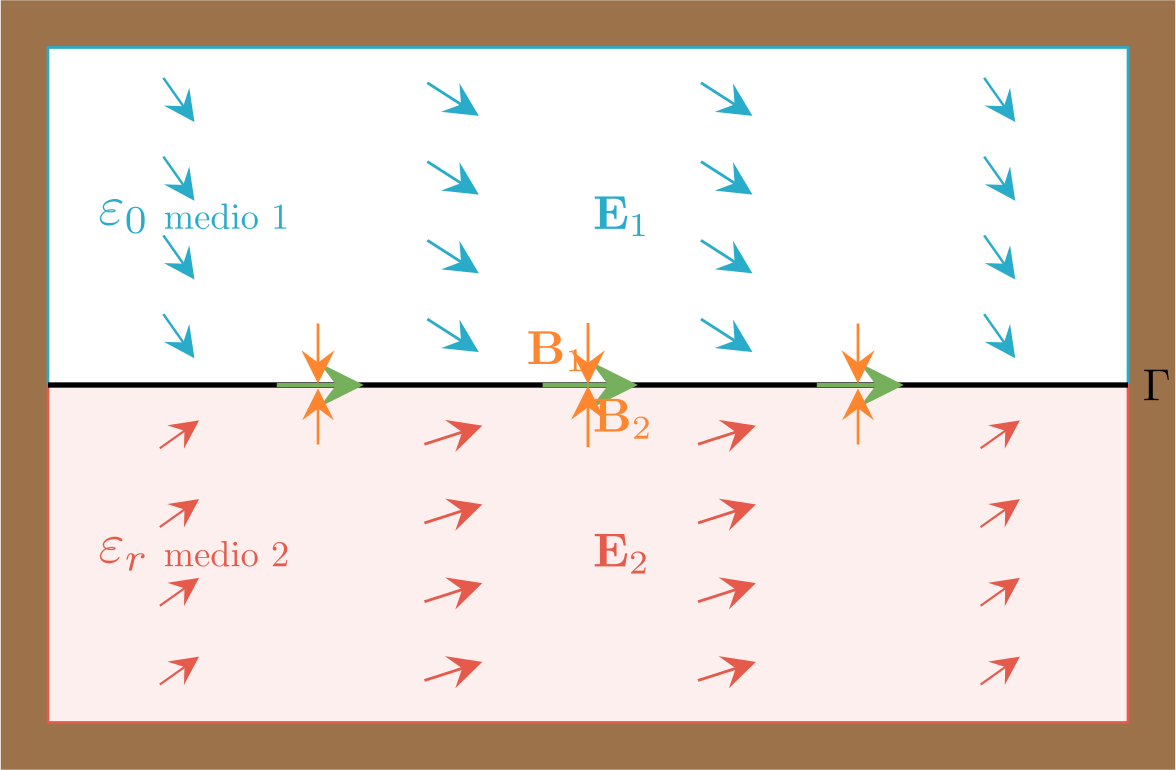
\includegraphics[width=\textwidth,height=0.30\textheight,keepaspectratio]{continuidad_dos_medios_2d.png}\\[0.9cm]
      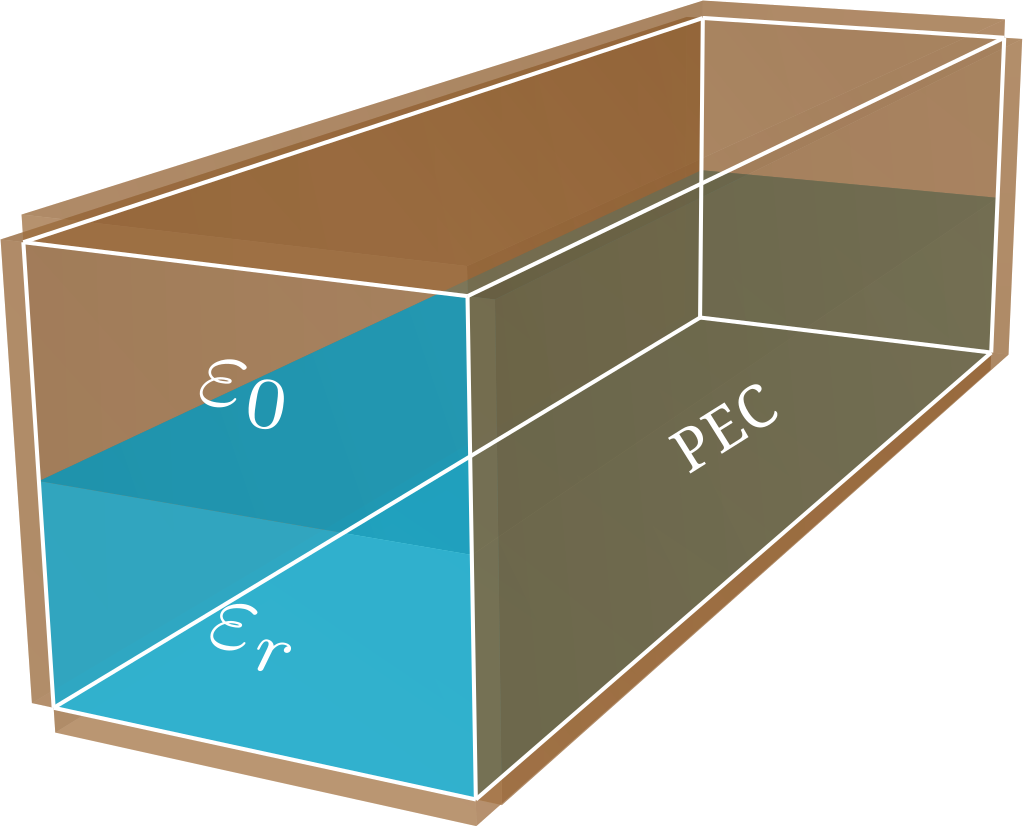
\includegraphics[width=\textwidth,height=0.34\textheight,keepaspectratio]{guia_onda_pec_white.png}
    \end{column}
  \end{columns}
\end{frame}

% ---------------------------------------------------------------------------
%  DIAPOSITIVA 12 — Problema de autovalores
% ---------------------------------------------------------------------------
\begin{frame}{Problema de autovalores}
  \vspace{-0.25cm}
  \setlength{\abovedisplayskip}{2pt}
  \setlength{\belowdisplayskip}{2pt}
  \begin{center}
  \begin{minipage}{0.94\textwidth}
    \small
    \textbf{1.} Un \textbf{autovalor} $\lambda$ con \textbf{autovector}
    $\mathbf{v}\neq\mathbf{0}$ cumple:
    \[
      \mathbf{A}\mathbf{v} = \lambda\mathbf{v}.
    \]
    \textbf{2.} Aquí el operador es $\mathbf{A}=\nabla\times\nabla\times$ y
    buscamos los campos $\mathbf{E}\neq\mathbf{0}$ y los valores admisibles de
    $k_0^2$. Imponiendo la condición de contorno PEC:
    \begin{block}{Problema de autovalores}
      \centering
      $\displaystyle
      \begin{aligned}
        \nabla \times \left( \frac{1}{\mu_r} \nabla \times \mathbf{E} \right)
          &= k_0^2\, \varepsilon_r\, \mathbf{E} \quad \text{en } \Omega, \\
        \hat{\mathbf{n}} \times \mathbf{E} &= \mathbf{0} \quad \text{en } \partial\Omega
      \end{aligned}$
    \end{block}
    \textbf{3.} Sus autovalores son los \textbf{modos de resonancia}
    $TE_{mn\ell}$ / $TM_{mn\ell}$ de la cavidad, y
    $k_0 = \omega\sqrt{\mu_0\varepsilon_0}$ relaciona el autovalor con la
    frecuencia.
  \end{minipage}
  \end{center}
\end{frame}

% ---------------------------------------------------------------------------
%  DIAPOSITIVA 12b — El problema de la forma fuerte
% ---------------------------------------------------------------------------
\begin{frame}{El problema de la forma fuerte}
  \vspace*{-0.4cm}
  \begin{center}
  \begin{minipage}{0.86\textwidth}
    \begin{block}{Problema modelo 1D}
      \centering
      $\displaystyle -u''(x) = f(x) \quad \text{en } (0,1),
        \qquad u(0) = u(1) = 0$
    \end{block}
  \end{minipage}
  \end{center}
  \vspace{0.7cm}
  \begin{columns}[T]
    \begin{column}{0.36\textwidth}
      \centering
      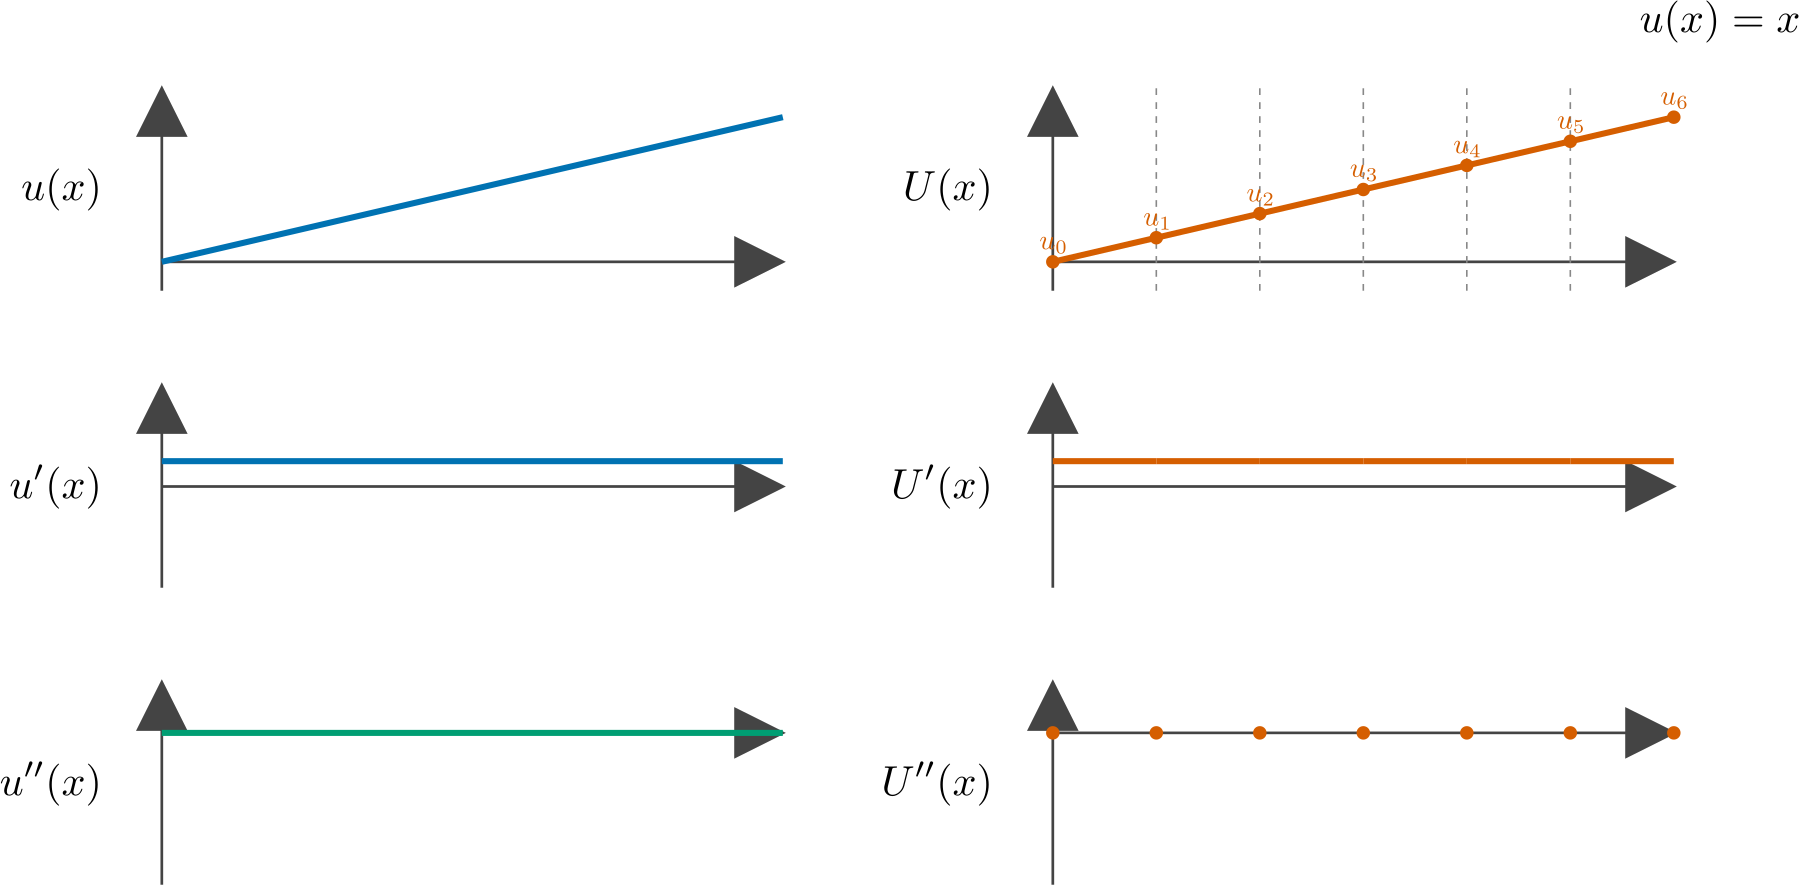
\includegraphics[width=\linewidth]{funcion_recta_white.png}\\[2pt]
      {\scriptsize $u(x)=x$}
    \end{column}
    \begin{column}{0.36\textwidth}
      \centering
      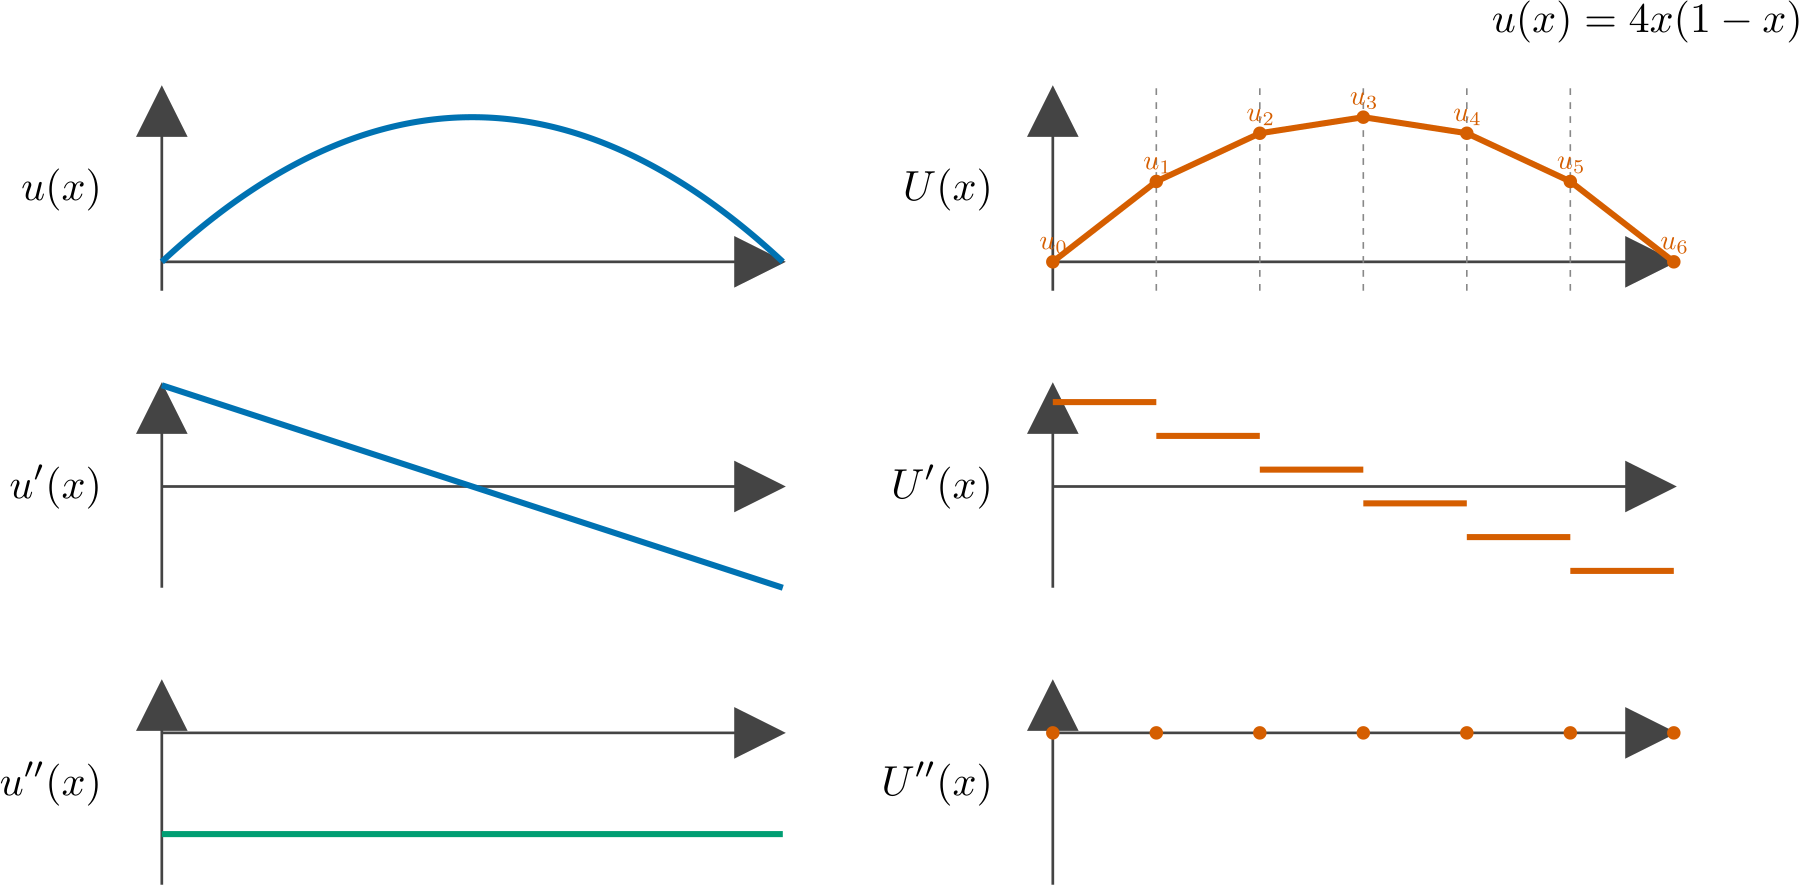
\includegraphics[width=\linewidth]{funcion_arco_white.png}\\[2pt]
      {\scriptsize $u(x)=4x(1-x)$}
    \end{column}
    \begin{column}{0.36\textwidth}
      \centering
      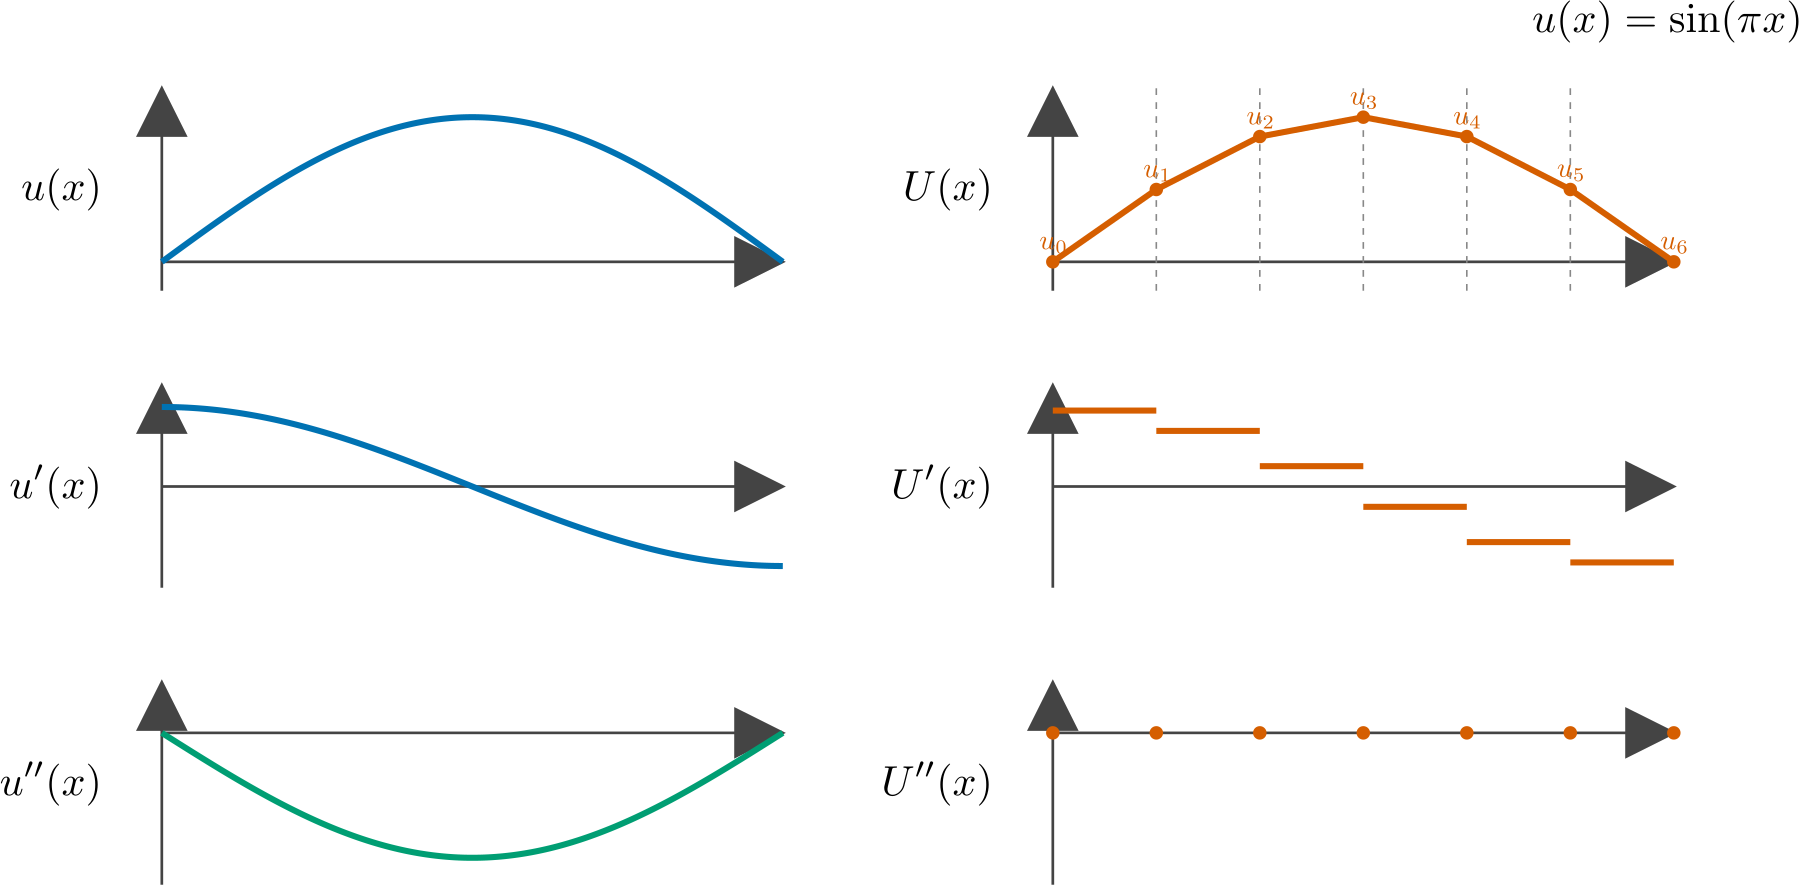
\includegraphics[width=\linewidth]{funcion_seno_white.png}\\[2pt]
      {\scriptsize $u(x)=\sin(\pi x)$}
    \end{column}
  \end{columns}
\end{frame}

% ===========================================================================
%  Diapositivas 12c-12g: formulación fuerte -> débil -> Hilbert
%  Paquetes necesarios en el preámbulo: amsmath, amssymb, graphicx
%  (con campos complejos, sustituir v por \bar{v} en las formas débiles)
% ===========================================================================

% ---------------------------------------------------------------------------
%  12c — De la forma fuerte a la débil: modelo 1D y nuestro problema
% ---------------------------------------------------------------------------
\begin{frame}[fragile]{De la forma fuerte a la formulación débil}
  \vspace{-0.40cm}
  \setlength{\abovedisplayskip}{2pt}
  \setlength{\belowdisplayskip}{2pt}
  \setlength{\jot}{0.5pt}
  \addtobeamertemplate{block begin}{\vspace{-3pt}}{}
  \addtobeamertemplate{block end}{\vspace{-3pt}}{}
  \begin{columns}[t]
  \begin{column}{0.98\textwidth}
    \scriptsize
    \begin{block}{Forma fuerte}
      \centering
      $\displaystyle
        \nabla\times\!\Big(\tfrac{1}{\mu_r}\,\nabla\times\mathbf{E}\Big)
        - k_0^2\,\varepsilon_r\,\mathbf{E} = \mathbf{0}
        \ \text{ en } \Omega$,
      \quad
      $\mathbf{n}\times\mathbf{E} = \mathbf{0}$ en $\partial\Omega$.
    \end{block}
    \vspace{0.10cm}
    \begin{itemize}\setlength\itemsep{3pt}
      \item \textbf{Paso 1.} Multiplicar por $\mathbf{v}$ e integrar en $\Omega$:
        \begin{center}
        $\displaystyle
          \int_\Omega \mathbf{v}\cdot\nabla\times\!\Big(\tfrac{1}{\mu_r}\nabla\times\mathbf{E}\Big)d\Omega
          - k_0^2\!\int_\Omega \varepsilon_r\,\mathbf{E}\cdot\mathbf{v}\,d\Omega = 0$
        \end{center}
      \item \textbf{Paso 2.} Integrar por partes el rotacional:
        \begin{center}
        $\displaystyle
          \int_\Omega \mathbf{v}\cdot\nabla\times\!\Big(\tfrac{1}{\mu_r}\nabla\times\mathbf{E}\Big)d\Omega
          = \int_\Omega \tfrac{1}{\mu_r}(\nabla\times\mathbf{E})\cdot(\nabla\times\mathbf{v})\,d\Omega
          - \oint_{\partial\Omega}\tfrac{1}{\mu_r}(\nabla\times\mathbf{E})\cdot(\mathbf{n}\times\mathbf{v})\,dS$
        \end{center}
      \item \textbf{Paso 3.} PEC anula el término de frontera
        ($\mathbf{n}\times\mathbf{E} = \mathbf{0}$ en $\partial\Omega$).
    \end{itemize}
    \vspace{0.10cm}
    \begin{block}{Forma débil: hallar $\mathbf{E}\in V$ tal que $\forall\,\mathbf{v}\in V$}
      \centering
      $\displaystyle
        \int_\Omega \tfrac{1}{\mu_r}(\nabla\times\mathbf{E})\cdot(\nabla\times\mathbf{v})\,d\Omega
        - k_0^2\!\int_\Omega \varepsilon_r\,\mathbf{E}\cdot\mathbf{v}\,d\Omega = 0$
    \end{block}
  \end{column}
  \end{columns}
\end{frame}

% ---------------------------------------------------------------------------
%  DIAPOSITIVA 13 — ¿Por qué elementos de Nédélec?
% ---------------------------------------------------------------------------
\begin{frame}{El espacio $H(\mathrm{curl})$ y los elementos de Nédélec}
  \vspace{0.15cm}
  \begin{columns}[t]
    \begin{column}{0.50\textwidth}
      \footnotesize
      \textbf{Problema.} Los elementos \textbf{nodales} imponen continuidad en
      las tres componentes del campo. Eso admite soluciones no físicas
      ($\mathbf{E}=\nabla\phi$, con $k_0^2=0$): los \textbf{modos espurios}.

      \vspace{0.15cm}
      \begin{block}{Solución: elementos de arista de Nédélec}
        \begin{itemize}\setlength\itemsep{1pt}
          \item Continuidad \textbf{solo tangencial}, no normal.
          \item Los campos irrotacionales ($\nabla\times\mathbf{E}=0$) quedan
            \textbf{aislados} en $k_0^2\approx 0$, lejos del espectro físico.
        \end{itemize}
      \end{block}

    \end{column}
    \begin{column}{0.48\textwidth}
      \centering
      \vspace{0.55cm}
      {\small\bfseries Espectro de $K$ (autovalores)}\\[0.25cm]
      % Figura original de la memoria (memoria/figuras/nucleo_K.png) sin texto.
      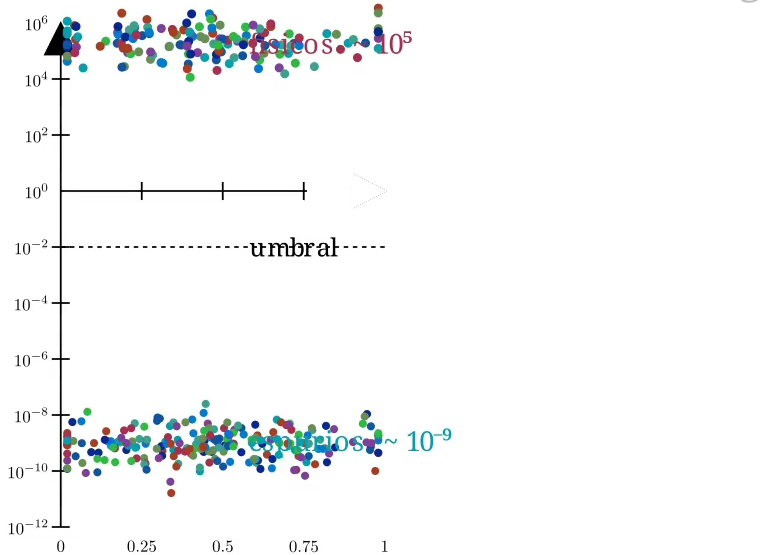
\includegraphics[width=\textwidth]{nucleo_K_white.png}
    \end{column}
  \end{columns}
  \vspace{0.1cm}
  \begin{center}
    \resizebox{\linewidth}{!}{%
      $P = \bigl\{ \mathbf{u} : u_1\in Q_{k-1,k,k},\;
        u_2\in Q_{k,k-1,k},\; u_3\in Q_{k,k,k-1} \bigr\}
      \;\Longrightarrow\;
      \ker(\mathbf{K}_h) = \nabla V_h^{\text{nodal}}$}
  \end{center}
\end{frame}

% ===========================================================================
\section{Implementación y validación}
% ===========================================================================

% ---------------------------------------------------------------------------
%  DIAPOSITIVA 14 — Portada de sección
% ---------------------------------------------------------------------------
\begin{frame}
  \sectionpage
\end{frame}

% ---------------------------------------------------------------------------
%  DIAPOSITIVA 14b — Diagrama de flujo de la estructura
% ---------------------------------------------------------------------------
\begin{frame}{Diagrama de flujo de la estructura}
  \vspace{-0.20cm}
  \begin{center}
  \hspace*{-0.35cm}%
  \resizebox{1.03\textwidth}{!}{%
  \begin{tikzpicture}[node distance=0.30cm and 0.28cm]
    % ------------------------------------------------------------------
    % Flujo interno del paquete NedelecHex (pipeline horizontal)
    % ------------------------------------------------------------------
    \node[etapa] (geo) {Geometría\\{\tiny ReferenceHex, Mesh}};
    \node[etapa, right=of geo] (mat) {Matemáticas\\{\tiny GaussQuadrature, CoordTransforms}};
    \node[etapa, right=of mat] (bas) {Bases\\{\tiny Monomials, DOFs, CoeffGen, BasisEval}};
    \node[etapa, right=of bas] (asm) {Ensamblaje\\{\tiny GlobalDOFs, Assembly}};
    \node[etapa, right=of asm] (res) {Resolución\\{\tiny eigs (ARPACK)}};
    \node[etapa, right=of res] (val) {Validación\\{\tiny test\_01..test\_10}};

    \draw[flujo] (geo) -- (mat);
    \draw[flujo] (mat) -- (bas);
    \draw[flujo] (bas) -- (asm);
    \draw[flujo] (asm) -- (res);
    \draw[flujo] (res) -- (val);

    % ------------------------------------------------------------------
    % Capa de integración (debajo del pipeline): el puente Julia--Fortran
    % es el intermediario entre NedelecHex y el simulador HOFEM.
    % ------------------------------------------------------------------
    \node[puente, below=1.15cm of asm] (bridge)
      {Puente Julia--Fortran\\{\tiny @ccall, cglobal, iso\_c\_binding}};
    \node[puente, left=0.9cm of bridge] (hofem)
      {HOFEM\\{\tiny simulador Fortran}\\[1pt]{\tiny (MPI + OpenMP)}};

    % El paquete se conecta con el puente, que lo integra en HOFEM.
    \draw[flujo] (bas.south) |- (bridge.north);
    \draw[flujo, <->] (bridge) -- node[etiq, above]{integración} (hofem);
  \end{tikzpicture}%
  }
  \end{center}
\end{frame}

% ---------------------------------------------------------------------------
%  DIAPOSITIVA 15 — Terna de Ciarlet
% ---------------------------------------------------------------------------
\begin{frame}{Terna de Ciarlet}
  Un elemento finito es la terna $(K, P_K, \Sigma_K)$:
  \begin{itemize}\setlength\itemsep{2pt}
    \item $K$: dominio simple, hexaedro de referencia $H = [0,1]^3$.
    \item $P_K$: espacio de funciones, $P_K = H_2$ (54 monomios).
    \item $\Sigma_K$: funcionales lineales (grados de libertad).
  \end{itemize}
  \vspace{0.15cm}
  \textbf{Cuatro etapas de FEM:}
  \begin{enumerate}\setlength\itemsep{2pt}
    \item Discretización del dominio.
    \item Funciones de interpolación.
    \item Sistema de ecuaciones.
    \item Resolución del sistema.
  \end{enumerate}
\end{frame}

% ---------------------------------------------------------------------------
%  DIAPOSITIVA 18 — Elemento de referencia
% ---------------------------------------------------------------------------
\begin{frame}{Elemento de referencia}
  \begin{columns}[c]
    \begin{column}{0.32\textwidth}
      \begin{itemize}
        \item Topología del hexaedro:
        \item Orden 2: $q \in Q_{2,2,2}$ $\Rightarrow$
          $\partial_\xi q \in Q_{1,2,2}$,
          $\partial_\eta q \in Q_{2,1,2}$,
          $\partial_\zeta q \in Q_{2,2,1}$
        \item $H_2 = Q_{1,2,2} \times Q_{2,1,2} \times Q_{2,2,1}$
        \item $\dim H_2 = 3 \cdot (2 \cdot 3 \cdot 3) = 54$
      \end{itemize}
    \end{column}
    \begin{column}{0.66\textwidth}
      \centering
      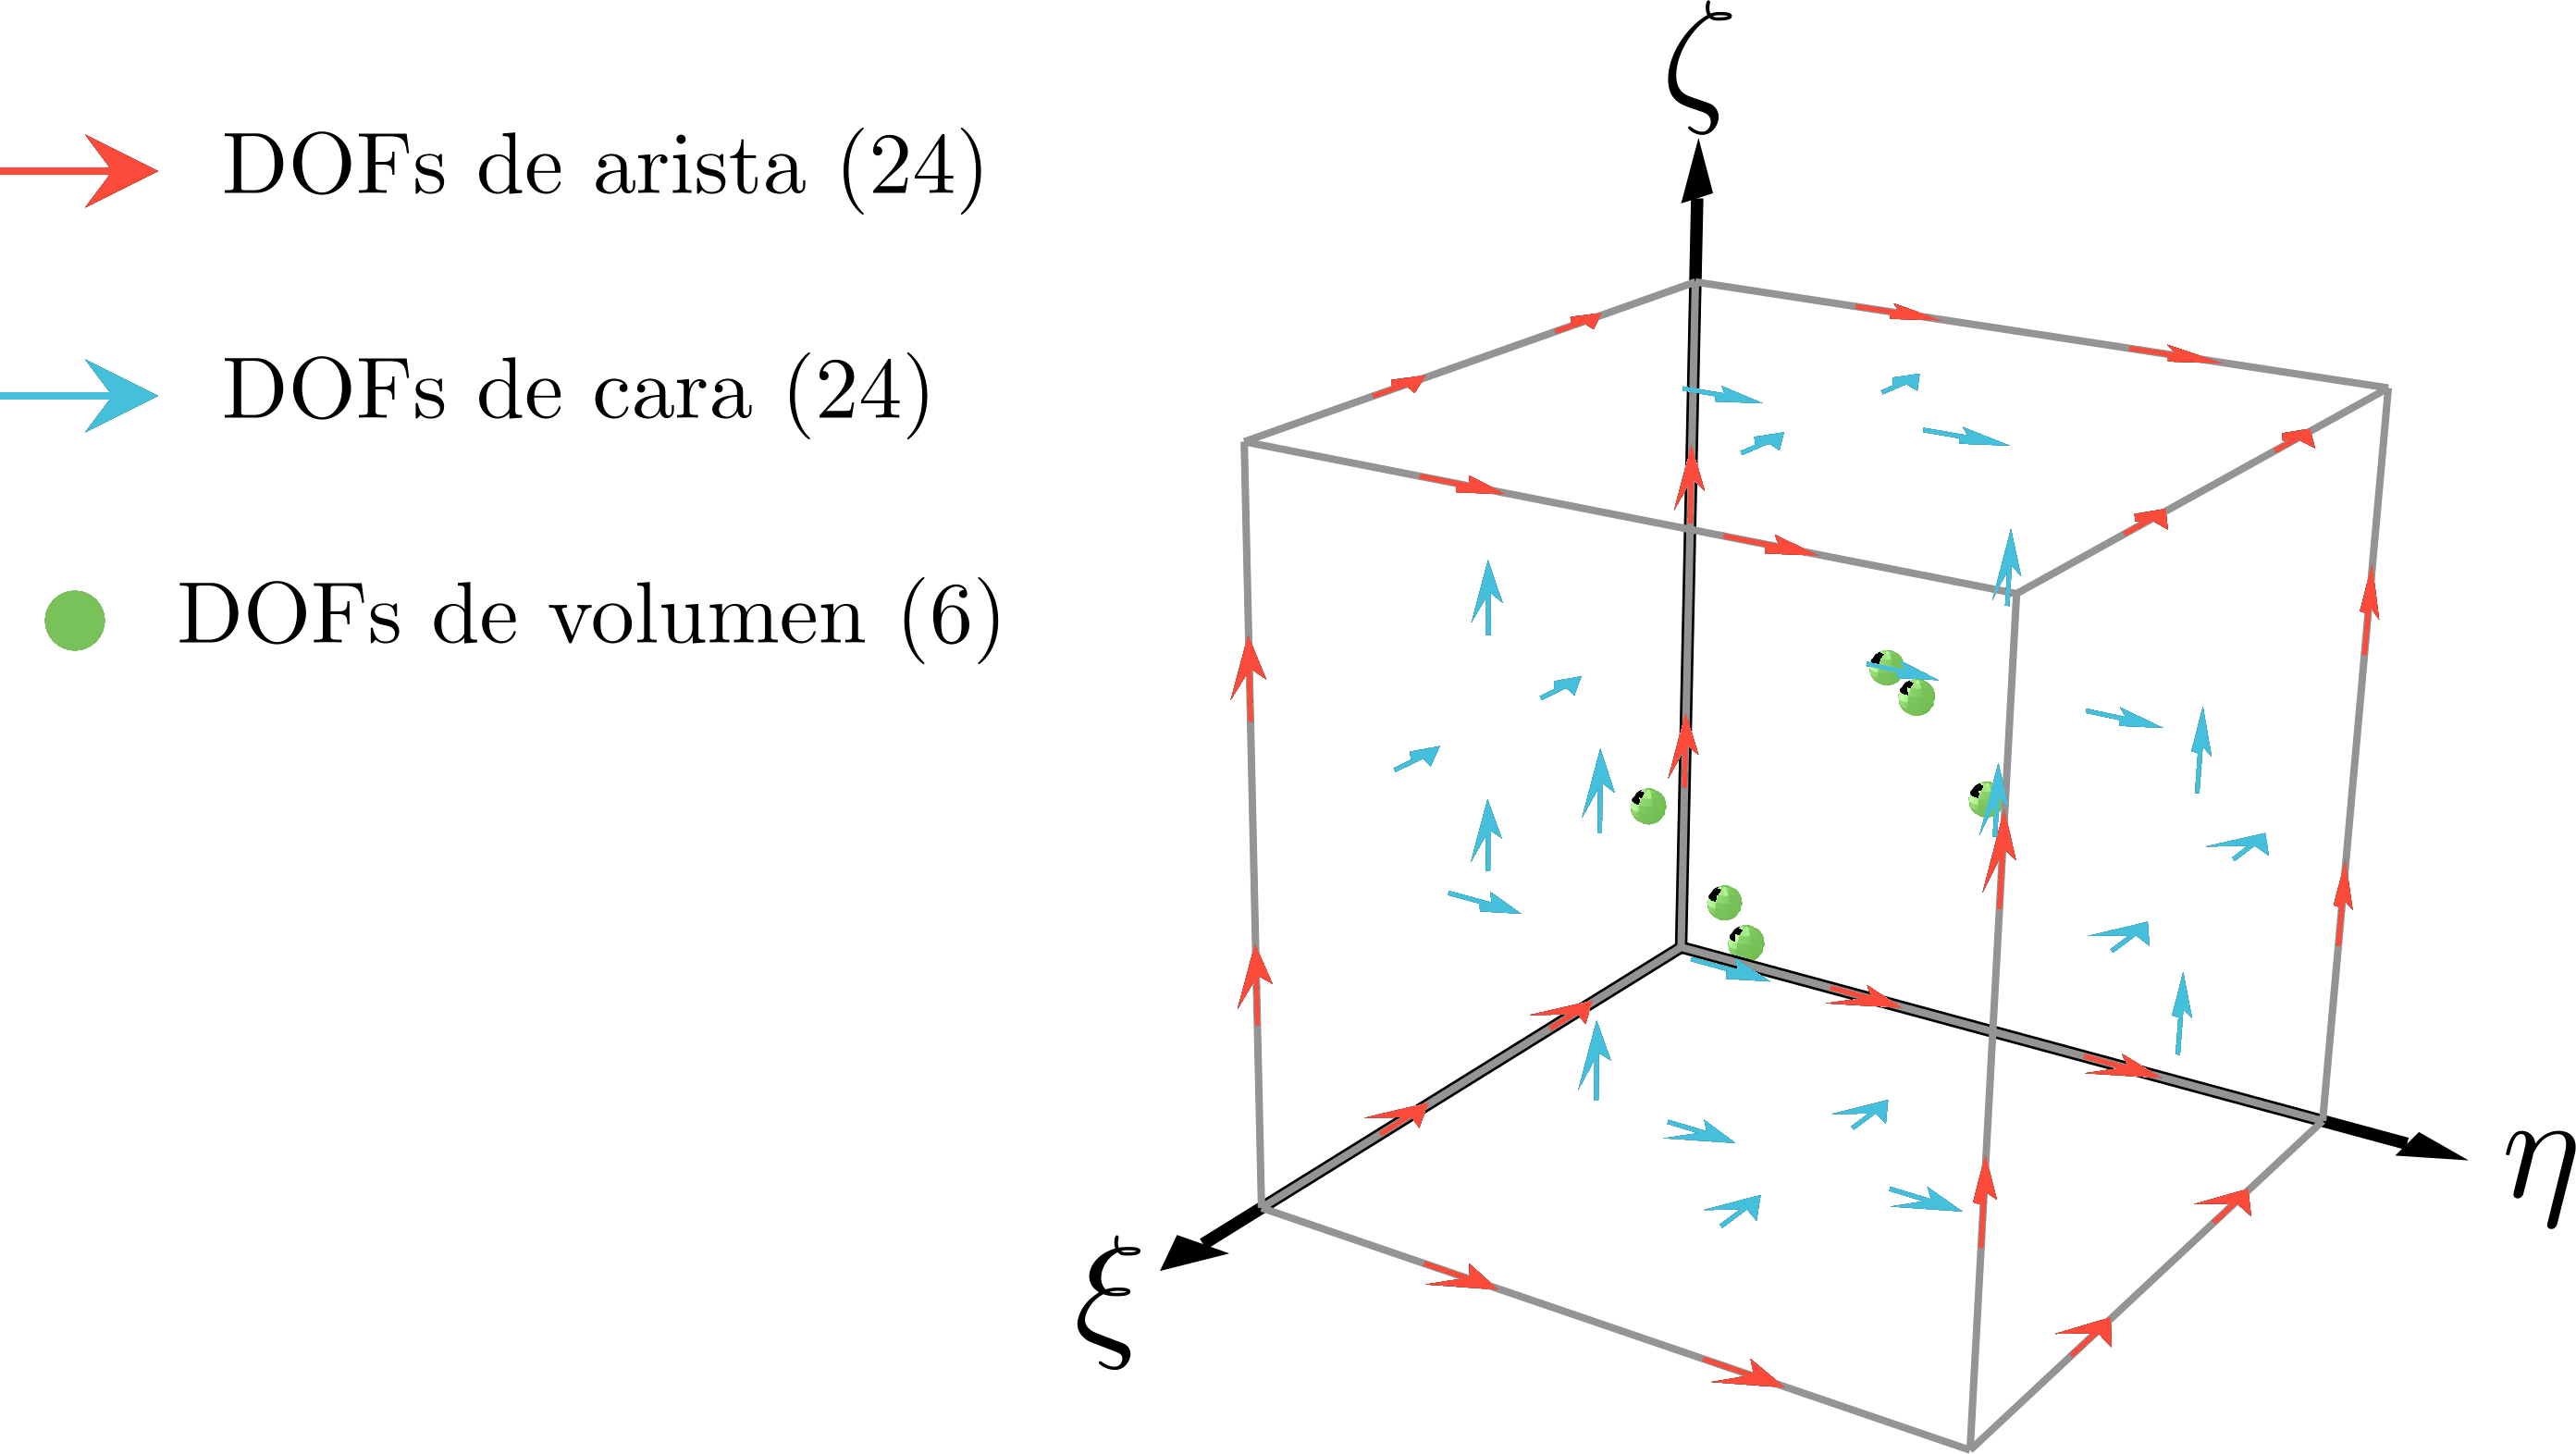
\includegraphics[width=\textwidth,height=0.85\textheight,keepaspectratio]{hexaedro_referencia_white.png}
    \end{column}
  \end{columns}
\end{frame}

% ---------------------------------------------------------------------------
%  DIAPOSITIVA 19 — Generación de los monomios
% ---------------------------------------------------------------------------
\begin{frame}{Generación de los monomios}
  El espacio de orden $k$ en el hexaedro de referencia $H=[0,1]^3$ es:
  \[
    \mathcal{H}_k =
    \begin{aligned}
      &\{P_{k-1}(I_\xi)\otimes P_k(I_\eta)\otimes P_k(I_\zeta)\}\\
      \times{}&\{P_k(I_\xi)\otimes P_{k-1}(I_\eta)\otimes P_k(I_\zeta)\}\\
      \times{}&\{P_k(I_\xi)\otimes P_k(I_\eta)\otimes P_{k-1}(I_\zeta)\}
    \end{aligned}
  \]
  Para orden $2$: $\mathcal{H}_2 = Q_{1,2,2} \times Q_{2,1,2} \times Q_{2,2,1}$,
  $\dim \mathcal{H}_2 = 3 \cdot (2\cdot3\cdot3) = 54$:
  \[
    \mathcal{H}_2 = \begin{pmatrix}
      a_1 + a_2\xi + a_3\eta + \cdots + a_{18}\xi\eta^2\zeta^2 \\
      b_1 + b_2\xi + b_3\xi^2 + \cdots + b_{18}\xi^2\eta\zeta^2 \\
      c_1 + c_2\xi + c_3\xi^2 + \cdots + c_{18}\xi^2\eta^2\zeta
    \end{pmatrix}
  \]
\end{frame}

% ---------------------------------------------------------------------------
%  DIAPOSITIVA 20 — 3 tipos de DOF
% ---------------------------------------------------------------------------
\begin{frame}{3 tipos de DOF}
  \begin{itemize}
    \item \textbf{Arista} (24 DOF): proyección sobre la tangente
      \[
        g_i^{\text{arista}}(\mathbf{u}) = \int_e (\mathbf{u} \cdot \hat{\tau})\,q\,dl,
        \qquad q \in \{1-t,\, t\}
      \]
    \item \textbf{Cara} (24 DOF): componente tangencial
      \[
        g_i^{\text{cara}}(\mathbf{u}) = \int_f (\hat{n} \times \mathbf{u}) \cdot \mathbf{q}\,ds,
        \qquad \mathbf{q} \in \{Q_{0,1} \times Q_{1,0}\}
      \]
    \item \textbf{Volumen} (6 DOF):
      \[
        g_i^{\text{vol}}(\mathbf{u}) = \int_H \mathbf{u} \cdot \mathbf{q}\,dV,
        \qquad \mathbf{q} \in \{Q_{1,0,0} \times Q_{0,1,0} \times Q_{0,0,1}\}
      \]
  \end{itemize}
  Total: $24 + 24 + 6 = 54$ DOF $= \dim H_2$.
\end{frame}

% ---------------------------------------------------------------------------
%  DIAPOSITIVA 21 — Generación de los coeficientes
% ---------------------------------------------------------------------------
\begin{frame}[fragile]{Generación de los coeficientes: la matriz de Gram $G$ y su inversa $W$}
  \vspace{-0.20cm}
  \setlength{\abovedisplayskip}{3pt}
  \setlength{\belowdisplayskip}{3pt}
  \setlength{\jot}{1pt}
  \begin{columns}[t]
  \begin{column}{0.42\textwidth}
    \scriptsize
    \textbf{Objetivo.} Buscamos la base dual $\{N_j\}_{j=1}^{54}\subset\mathcal{H}_2$ tal que
    $\;g_i(N_j) = \delta_{ij},\quad i,j=1,\dots,54$.

    \vspace{0.10cm}
    \textbf{Paso 1.} Cada $N_j$ es combinación lineal de los monomios $u_k$:
    \[
      \mathbf{N}_j = \sum_{k=1}^{54} W_{kj}\,u_k
    \]

    \textbf{Paso 2.} Aplicando los funcionales y usando $G_{ij}=g_i(u_j)$:
    \[
      g_i(\mathbf{N}_j) = \sum_{k=1}^{54} W_{kj}\,g_i(u_k)
      = \sum_{k=1}^{54} W_{kj}\,G_{ik}
      = (\mathbf{G}\mathbf{W})_{ij} = \delta_{ij}
    \]

    \textbf{Paso 3.} Invertimos la matriz de Gram:
    \[
      \mathbf{G}\,\mathbf{W} = \mathbf{I}_{54}
      \quad\Longrightarrow\quad
      \mathbf{W} = \mathbf{G}^{-1}
    \]
  \end{column}
  \hfill
  \begin{column}{0.52\textwidth}
    \begin{flushright}
    \begin{lstlisting}[style=codestyle,basicstyle=\ttfamily\fontsize{6}{7}\selectfont]
function get_coefficients()
    monomials = build_h2_monomials()
    N = length(monomials)
    G = zeros(N, N)
    for j in 1:N
        G[:, j] = evaluate_all_dofs(monomials[j])
    end
    W = G \ I(N)
    return W, G
end
    \end{lstlisting}
    \end{flushright}
  \end{column}
  \end{columns}
\end{frame}

% ---------------------------------------------------------------------------
%  DIAPOSITIVA 22 — Mapeo al elemento real y etiquetado
% ---------------------------------------------------------------------------
\begin{frame}{Mapeo al elemento real y etiquetado}
  \begin{columns}[c]
    \begin{column}{0.42\textwidth}
      \textbf{Mapeo isoparamétrico:}
      \[
        x = \sum_{i=1}^{n_e} N_i^e(\xi,\eta,\zeta)\,x_i
      \]
      \textbf{Transformaciones de Piola:}
      \[
        \underbrace{\mathbf{N} = J^{-T}\hat{\mathbf{N}}}_{\text{covariante}}
      \]
      \[
        \underbrace{\nabla \times \mathbf{N} = \frac{1}{\det J}\,J\,(\hat{\nabla} \times \hat{\mathbf{N}})}_{\text{contravariante}}
      \]
    \end{column}
    \begin{column}{0.56\textwidth}
      \centering
      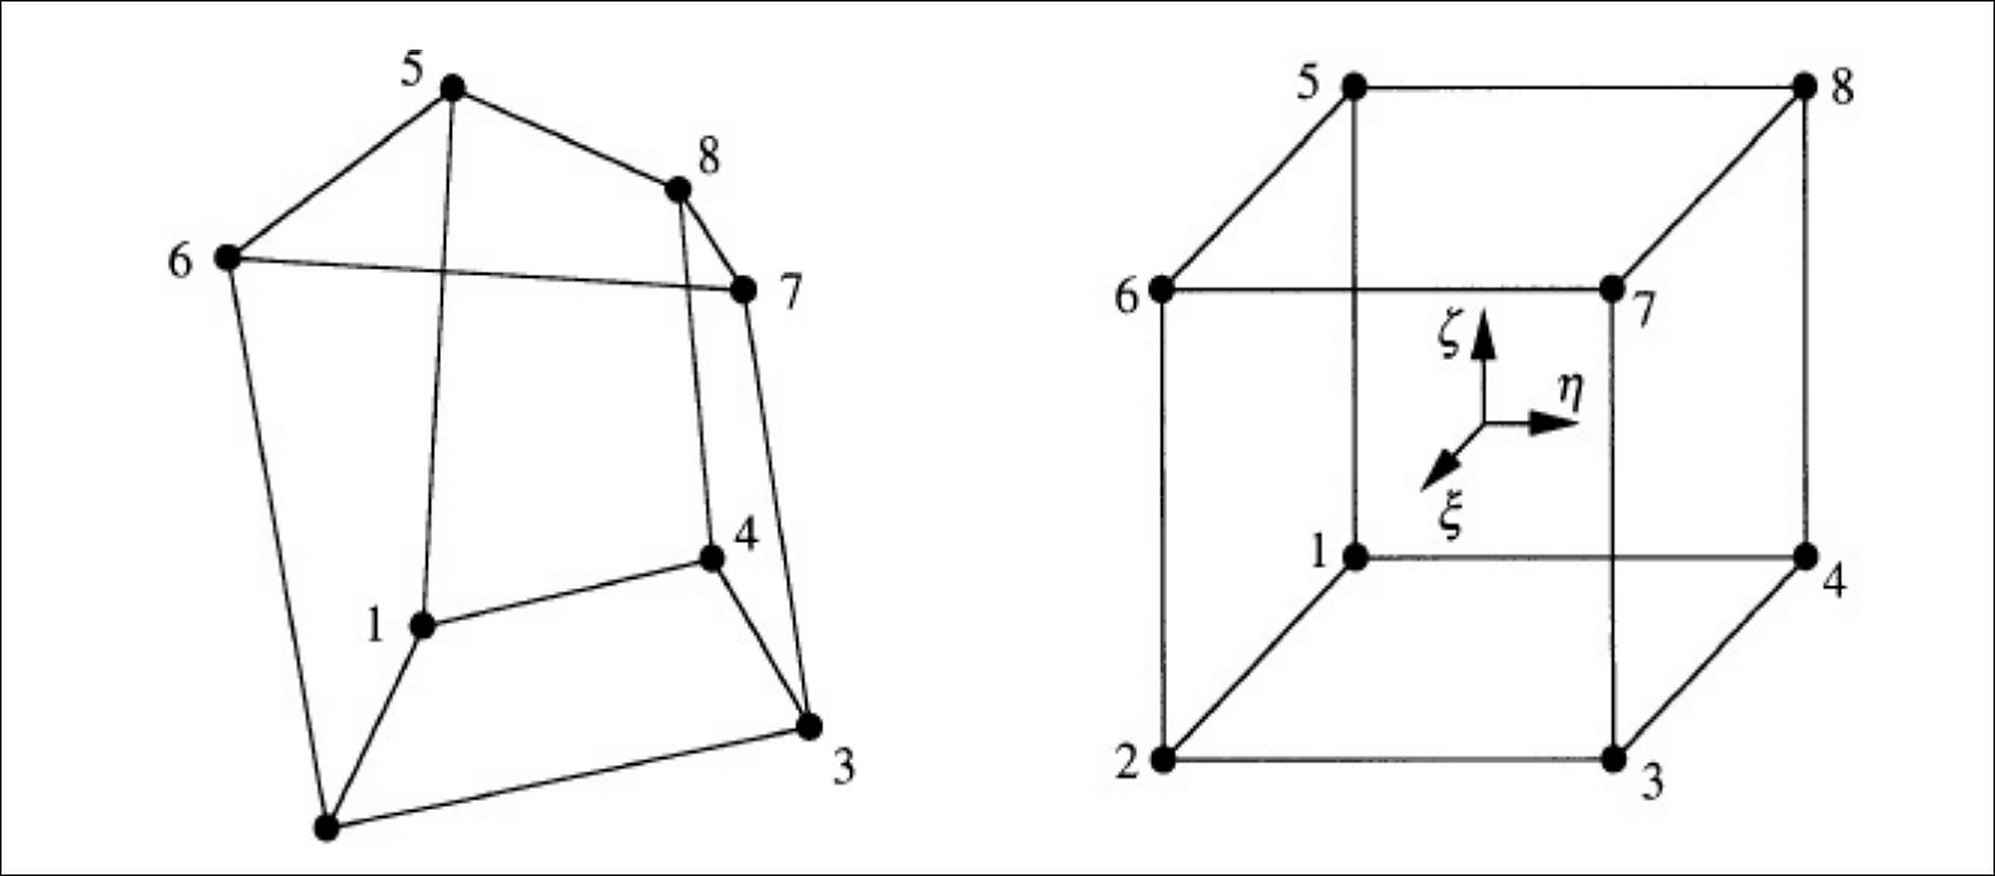
\includegraphics[width=\textwidth]{jianming_jin_upscaled.png}
    \end{column}
  \end{columns}
\end{frame}

% ---------------------------------------------------------------------------
%  DIAPOSITIVA 23 — Ensamblaje del sistema
% ---------------------------------------------------------------------------
\begin{frame}{Ensamblaje del sistema}
  \vspace{-0.4cm}
  Campo como combinación de las 54 bases:
  $\mathbf{E}_h = \sum_{j=1}^{54} x_j \mathbf{N}_j$.
  \begin{center}
  \begin{minipage}{0.92\textwidth}
    \begin{center}
      $\scriptstyle
      \sum_{j=1}^{54} x_j \int_{\Omega_e} \frac{1}{\mu_r}
      (\nabla \times \mathbf{N}_j) \cdot (\nabla \times \mathbf{N}_i)\,d\Omega
      - k_0^2 \sum_{j=1}^{54} x_j \int_{\Omega_e} \varepsilon_r\,
      \mathbf{N}_j \cdot \mathbf{N}_i\,d\Omega = 0$
    \end{center}
    \begin{block}{Matrices elementales}
      \centering
      $\small
      \begin{aligned}
        K_{ij}^e &= \int_{\Omega_e} \frac{1}{\mu_r}
          (\nabla \times \mathbf{N}_i) \cdot (\nabla \times \mathbf{N}_j)\,d\Omega, \\
        M_{ij}^e &= \int_{\Omega_e} \varepsilon_r\,
          \mathbf{N}_i \cdot \mathbf{N}_j\,d\Omega
      \end{aligned}$
    \end{block}
  \end{minipage}
  \end{center}
  \vspace{-0.2cm}
  \begin{itemize}\setlength\itemsep{0pt}
    \item $K^e$: cuánto se ``enrollan'' las bases (campo magnético).
    \item $M^e$: cuánto se solapan (campo eléctrico).
    \item Las bases con geometrías compartidas tienen el mismo DOF.
  \end{itemize}
\end{frame}

% ---------------------------------------------------------------------------
%  DIAPOSITIVA 24 — Resolución del sistema
% ---------------------------------------------------------------------------
\begin{frame}{Resolución del sistema}
  \begin{center}
  \begin{minipage}{0.86\textwidth}
    \begin{block}{Problema de autovalores generalizado}
      \centering
      $\displaystyle K\mathbf{x} = k_0^2 M\mathbf{x}$
    \end{block}
  \end{minipage}
  \end{center}
  \begin{itemize}\setlength\itemsep{2pt}
    \item $\lambda = k_0^2$: frecuencias de resonancia de la cavidad.
    \item $\mathbf{x}$: coeficientes de cada modo en la base de Nédélec.
    \item $K$ singular: $\ker(K_h) = \nabla V_h^{\text{nodal}}$.
    \item Modos espurios en $k_0^2 \approx 0$, separados del espectro físico.
    \item Resuelto con ARPACK (\texttt{eigs}) cerca de un desplazamiento $\sigma$.
  \end{itemize}
\end{frame}

% ---------------------------------------------------------------------------
%  DIAPOSITIVA 26 — Validación numérica
% ---------------------------------------------------------------------------
\begin{frame}{Validación numérica}
  \begin{columns}[T]
    \begin{column}{0.40\textwidth}
      \vspace{0.1cm}
      \footnotesize
      \begin{itemize}\setlength\itemsep{4pt}
        \item Coeficientes: $W = G^{-1}$ entera
        \item Núcleos: $\dim\ker(K)$ correcta
        \item $K$ y $M$: coinciden con MATLAB
        \item Autovalores: error medio $3{,}1\cdot10^{-5}$ (malla 5)
        \item Pendientes: $4{,}61$ (semillena) y $4{,}76$ (vacía) frente a $4$ teórico
      \end{itemize}
    \end{column}
    \begin{column}{0.58\textwidth}
      \centering
      \vfill
      {\small\bfseries Convergencia de autovalores}\\[4pt]
      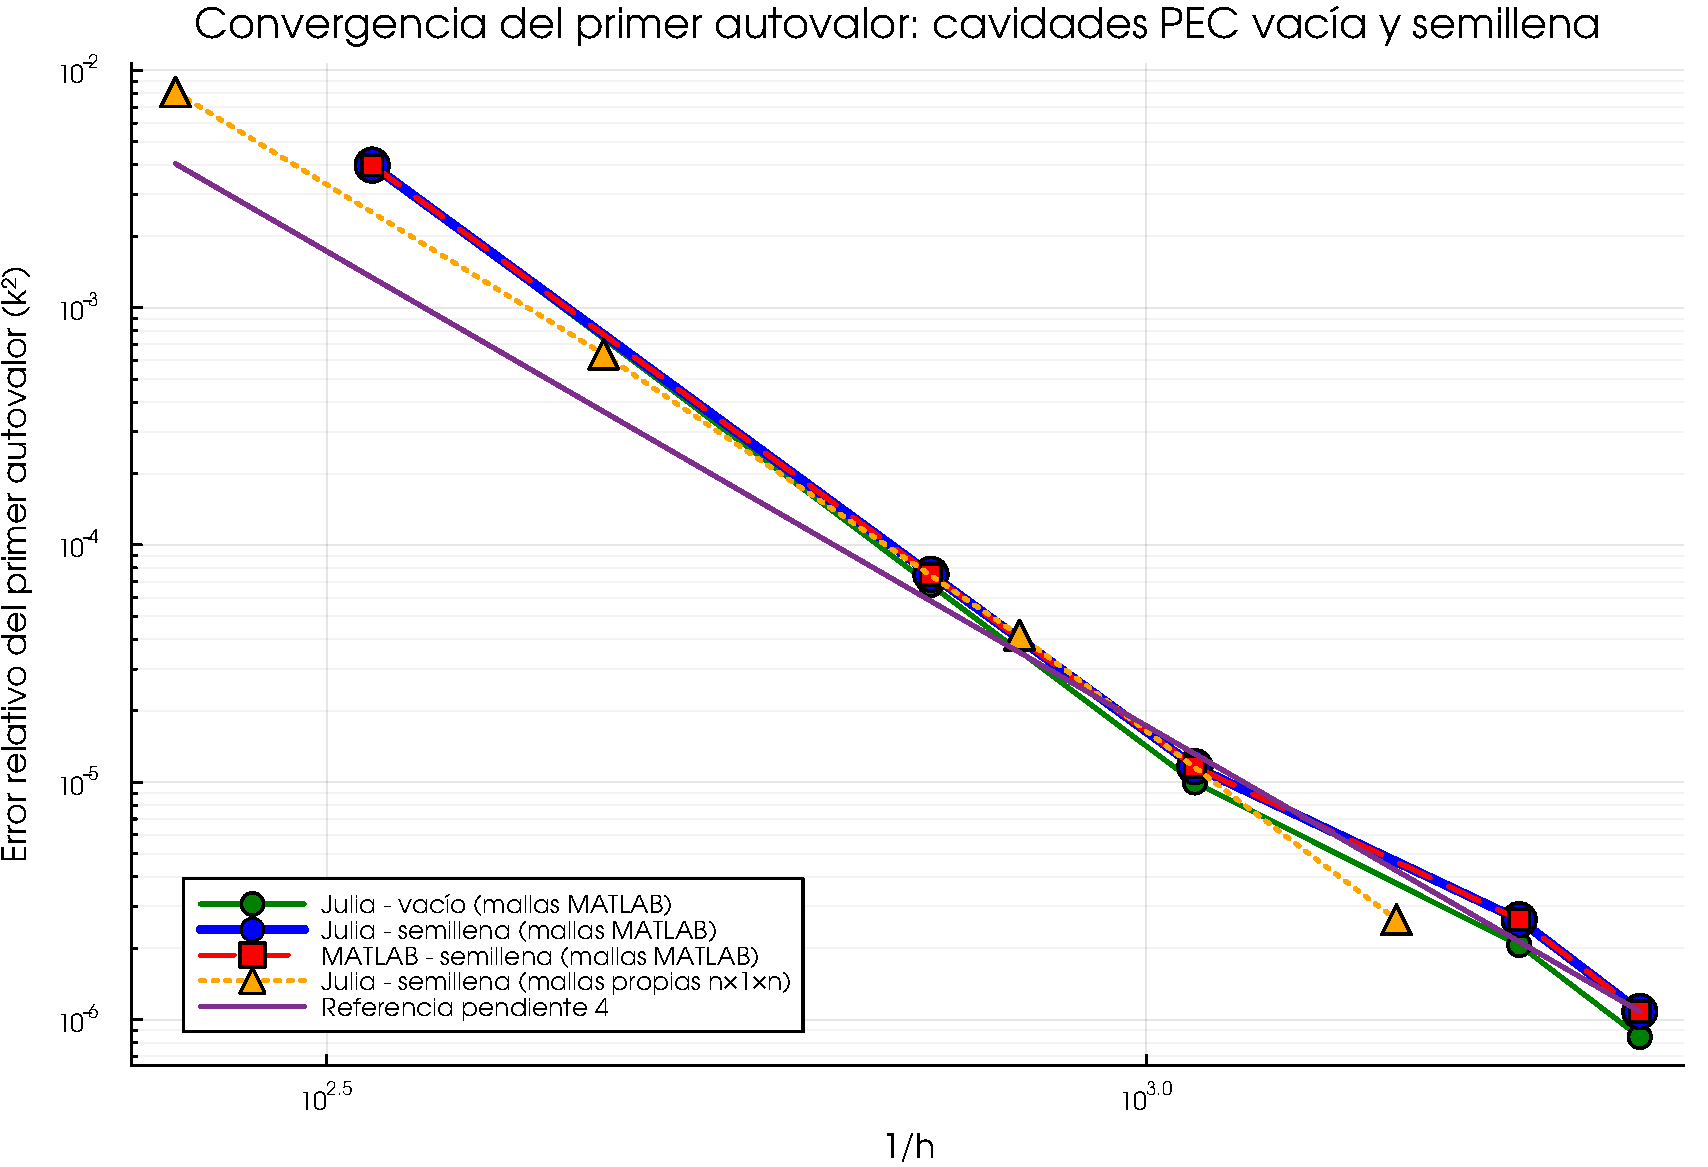
\includegraphics[width=\linewidth,height=0.62\textheight,keepaspectratio]{convergencia_combinada_cavidades.pdf}
      \vfill
    \end{column}
  \end{columns}
\end{frame}

% ---------------------------------------------------------------------------
%  DIAPOSITIVA 27 — Comparación de rendimiento y de memoria
% ---------------------------------------------------------------------------
\begin{frame}{Comparación de rendimiento y de memoria}
  \vspace{-0.35cm}
  \begin{center}
    \footnotesize
    \begin{tabular}{lrrr}
      \hline
      \textbf{Etapa} & \textbf{Julia} & \textbf{MATLAB} & \textbf{Cociente}\\
      \hline
      Coeficientes            & 4{,}5 ms    & 251{,}0 ms   & $\mathbf{56}$\\
      Numeración de DOF       & 1{,}0 ms    & 28{,}3 ms    & $\mathbf{30}$\\
      Ensamblaje + Dirichlet  & 1199{,}4 ms & 17136{,}7 ms & $\mathbf{14}$\\
      Resolución              & 391{,}8 ms  & 424{,}2 ms   & $1{,}1$\\
      \hline
    \end{tabular}
  \end{center}
  \vspace{0.1cm}
  \begin{itemize}\setlength\itemsep{2pt}
    \item Malla de 23124 DOF, 1 hilo en ambos lenguajes.
    \item Construcción del sistema: $14\times$--$56\times$ más rápida en Julia.
    \item \textbf{Solver} comparable (ambos usan ARPACK).
    \item Memoria de $K$ y $M$ equivalente.
  \end{itemize}
\end{frame}

% ===========================================================================
\section{Resultados y conclusiones}
% ===========================================================================

% ---------------------------------------------------------------------------
%  DIAPOSITIVAS 29a–29d — Uso del paquete NedelecHex (4 pasos progresivos)
%  Cada diapositiva muestra el mismo código completo; el bloque activo va
%  subrayado y el título indica qué hace ese bloque.
% ---------------------------------------------------------------------------
% (El estilo \texttt{codestyle} se define en el preámbulo.)

% Macro para resaltar el bloque activo: color de acento + negrita, sin subrayar.
\newcommand{\hl}[1]{\textcolor{red!80!black}{\textbf{#1}}}

% ── Paso 1: malla y etiquetado (solo se muestra el primer bloque) ───────────
\begin{frame}[fragile]{Uso del paquete: malla y etiquetado}
\vspace{-0.15cm}
\begin{lstlisting}[style=codestyle]
(*\hl{using NedelecHex}*)
(*\hl{mesh = box\_mesh(Lx=0.01, Ly=0.001,}*)
(*\hl{\ \ \ \ \ \ \ \ Lz=0.01, nx=8, ny=1, nz=8)}*)
(*\hl{tag\_solids\_by\_plane!(mesh; axis=:z, cut=0.005)}*)
(*\hl{tag\_exterior\_boundary!(mesh; type="PerfectE")}*)
\end{lstlisting}
\end{frame}

% ── Paso 2: + grados de libertad y bases ────────────────────────────────────
\begin{frame}[fragile]{Uso del paquete: grados de libertad y bases}
\addtocounter{framenumber}{-1}
\vspace{-0.15cm}
\begin{lstlisting}[style=codestyle]
using NedelecHex
mesh = box_mesh(Lx=0.01, Ly=0.001,
                Lz=0.01, nx=8, ny=1, nz=8)
tag_solids_by_plane!(mesh; axis=:z, cut=0.005)
tag_exterior_boundary!(mesh; type="PerfectE")

(*\hl{dof\_map = build\_dof\_map(mesh)}*)
(*\hl{W, \_ = get\_coefficients()}*)
(*\hl{mono = build\_h2\_monomials()}*)
(*\hl{curl = build\_h2\_curl\_monomials()}*)
\end{lstlisting}
\end{frame}

% ── Paso 3: + ensamblaje ────────────────────────────────────────────────────
\begin{frame}[fragile]{Uso del paquete: ensamblaje}
\addtocounter{framenumber}{-1}
\vspace{-0.15cm}
\begin{lstlisting}[style=codestyle]
using NedelecHex
mesh = box_mesh(Lx=0.01, Ly=0.001,
                Lz=0.01, nx=8, ny=1, nz=8)
tag_solids_by_plane!(mesh; axis=:z, cut=0.005)
tag_exterior_boundary!(mesh; type="PerfectE")

dof_map = build_dof_map(mesh)
W, _ = get_coefficients()
mono = build_h2_monomials()
curl = build_h2_curl_monomials()

(*\hl{K, M = assemble\_global\_matrices(mesh, dof\_map,}*)
(*\hl{\ \ \ \ \ \ \ \ \ \ W, mono, curl; dirichlet=true)}*)
\end{lstlisting}
\end{frame}

% ── Paso 4: ejemplo de uso completo ─────────────────────────────────────────
\begin{frame}[fragile]{Uso del paquete: ejemplo completo}
\addtocounter{framenumber}{-1}
\vspace{-0.15cm}
\begin{lstlisting}[style=codestyle]
using NedelecHex

# 1. Malla y etiquetado
mesh = box_mesh(Lx=0.01, Ly=0.001,
                Lz=0.01, nx=8, ny=1, nz=8)
tag_solids_by_plane!(mesh; axis=:z, cut=0.005)
tag_exterior_boundary!(mesh; type="PerfectE")

# 2. Grados de libertad y bases
dof_map = build_dof_map(mesh)
W, _ = get_coefficients()
mono = build_h2_monomials()
curl = build_h2_curl_monomials()

# 3. Ensamblaje del sistema
K, M = assemble_global_matrices(mesh, dof_map,
          W, mono, curl; dirichlet=true)
\end{lstlisting}
\end{frame}

% ---------------------------------------------------------------------------
%  DIAPOSITIVA 31 — Conclusiones
% ---------------------------------------------------------------------------
\begin{frame}{Conclusiones}
  \begin{itemize}
    \item \textbf{O1--O2.} Funciones de base y coeficientes implementados y verificados
    \item \textbf{O3.} Ensamblaje global validado: dimensión del núcleo de $K$
      correcta y matrices $K$, $M$ coincidentes con MATLAB
    \item \textbf{O4.} Benchmark de la cavidad semillena reproducido con convergencia
    \item \textbf{O5.} Julia $14$--$56\times$ más rápida en la construcción del sistema; solver equivalente (ARPACK)
    \item Líneas futuras: generalizar condiciones de contorno y más topologías
  \end{itemize}
\end{frame}

% ---------------------------------------------------------------------------
%  DIAPOSITIVA 32 — ¡Gracias!
% ---------------------------------------------------------------------------
\begin{frame}
  \begin{center}
    {\Huge ¡Gracias!}
  \end{center}
  % Etiqueta de la última diapositiva principal: el pie la usa para el total
  % de la parte principal (sin anexos). Debe ir DENTRO del frame para que
  % Beamer capture el número de diapositiva correcto.
  \label{lastmainframe}
\end{frame}

\appendix
% A partir de aquí empiezan los anexos: reiniciamos el contador de diapositiva
% y activamos el indicador \ifanexos para que el pie numere los anexos aparte
% («actual / total de anexos») sin mezclarlos con las diapositivas principales.
\anexostrue
\setcounter{framenumber}{0}
\section{Anexos}
% ===========================================================================

% ---------------------------------------------------------------------------
%  DIAPOSITIVA A1 — Portada del anexo
% ---------------------------------------------------------------------------
\begin{frame}
  \begin{center}
    {\Large\textbf{Anexos}}\\[0.6cm]
    {\normalsize Suite de verificación: 10 ficheros de test en Julia}
  \end{center}
\end{frame}

% ---------------------------------------------------------------------------
%  DIAPOSITIVA A2 — La suite de tests: visión general
% ---------------------------------------------------------------------------
\begin{frame}{Anexo: suite de verificación (\texttt{NedelecHex/test/})}
  \small
  \begin{columns}[T]
    \begin{column}{0.56\textwidth}
      \textbf{10 ficheros:}
      \begin{enumerate}\setlength\itemsep{1pt}\scriptsize
        \item \texttt{test\_01\_quadrature.jl}
        \item \texttt{test\_02\_monomials.jl}
        \item \texttt{test\_03\_dofs.jl}
        \item \texttt{test\_04\_coefficients.jl}
        \item \texttt{test\_05\_reference\_element.jl}
        \item \texttt{test\_06\_gmsh\_node\_order.jl}
        \item \texttt{test\_07\_bases\_eval.jl}
        \item \texttt{test\_08\_assembly.jl}
        \item \texttt{test\_09\_tags.jl}
        \item \texttt{test\_10\_half\_filled\_cavity.jl}
      \end{enumerate}
    \end{column}
    \begin{column}{0.42\textwidth}
      \textbf{Ejecución:}\\[2pt]
      {\ttfamily\scriptsize julia --project=.}\\
      {\ttfamily\scriptsize \hspace*{1em}test/runtests.jl}\\[6pt]
      \textbf{Verbose} (añade explicaciones):\\[2pt]
      {\ttfamily\scriptsize NEDELEC\_TEST\_VERBOSE=1}\\
      {\ttfamily\scriptsize julia --project=.}\\
      {\ttfamily\scriptsize \hspace*{1em}test/runtests.jl}\\[6pt]
      \textbf{Omitir tests} concretos:\\[2pt]
      {\ttfamily\scriptsize NEDELEC\_TEST\_SKIP=\char`\"06,09\char`\"}\\
      {\ttfamily\scriptsize julia --project=.}\\
      {\ttfamily\scriptsize \hspace*{1em}test/runtests.jl}
    \end{column}
  \end{columns}
\end{frame}

% ---------------------------------------------------------------------------
%  DIAPOSITIVA A3 — Tests 01-04: infraestructura matemática
% ---------------------------------------------------------------------------
\begin{frame}{Anexo: tests 01--04 (infraestructura matemática)}
  \small
  \begin{description}\setlength\itemsep{3pt}
    \item[\texttt{test\_01} Cuadratura de Gauss.]
      Reglas 1D/2D/3D: $\sum w = 1$ (partición del volumen unidad) y
      exactitud polinómica $\int \xi^2\eta^2\zeta^2\,dV = 1/27$.
      La regla 3D de orden 4 usa $3^3 = 27$ puntos.
    \item[\texttt{test\_02} Los 54 monomios de $H_2$.]
      $54 = 3 \times 18$ bloques ($\hat\xi,\hat\eta,\hat\zeta$); cada monomio
      tiene una única componente no nula. Se verifica el grado polinómico
      con diferencias finitas (grado $\le 1$ en su variable, $\le 2$ en las
      demás).
    \item[\texttt{test\_03} Funcionales DOF.]
      Integrales de arista, cara y volumen contra valores calculados a mano
      (p.\,ej.\ $g_1 = \int_0^1 t^2(1-t)\,dt = 1/12$). Comprueba también
      DOFs nulos por ortogonalidad y por anulación geométrica.
    \item[\texttt{test\_04} Matriz $G$ y coeficientes $W$.]
      $\mathrm{rank}(G) = 54$ (unisolvencia), $\mathrm{cond}(G) < 10^5$,
      $G\,W = I_{54}$, $W$ entera con $|W_{ij}| \le 216$ y coincidencia
      exacta con la Tabla II del paper.
  \end{description}
\end{frame}

% ---------------------------------------------------------------------------
%  DIAPOSITIVA A4 — Tests 05-07: elemento de referencia y malla
% ---------------------------------------------------------------------------
\begin{frame}{Anexo: tests 05--07 (elemento de referencia y malla)}
  \small
  \begin{description}\setlength\itemsep{3pt}
    \item[\texttt{test\_05} Elemento de referencia.]
      Jacobiano $J = I_3$ en el hexaedro sin deformar y $J = \mathrm{diag}(a,b,c)$
      en un ladrillo escalado; propiedad dual $g_i(N_j) = \delta_{ij}$ evaluando
      las bases reales; $\mathrm{curl} \neq 0$ en las 6 bases de volumen y
      caracterización de los modos irrotacionales (espurios).
    \item[\texttt{test\_06} Permutación de nodos de Gmsh.]
      Genera una malla con Gmsh ``en crudo'' y comprueba que el orden de nodos
      no coincide con \texttt{ReferenceHex.NODES} hasta aplicar la permutación
      \texttt{[3,7,8,4,2,6,5,1]}.
    \item[\texttt{test\_07} Bases evaluadas vs MATLAB.]
      Reproduce la comparación triple de \texttt{mainEvaluateCoefficients.m}:
      Tabla II simbólica / código MATLAB / Julia, en el punto central
      $(0.5,0.5,0.5)$ del hexaedro de referencia.
  \end{description}
\end{frame}

% ---------------------------------------------------------------------------
%  DIAPOSITIVA A5 — Tests 08-10: ensamblaje y verificación física
% ---------------------------------------------------------------------------
\begin{frame}{Anexo: tests 08--10 (ensamblaje y física)}
  \small
  \begin{description}\setlength\itemsep{3pt}
    \item[\texttt{test\_08} Ensamblaje global.]
      Mallas $1 \to 2 \to 8$ elementos; dimensión del núcleo de $K$
      (modos gradiente espurios) $26 / 44 / 124$; DOFs compartidos entre
      elementos adyacentes ($54+54-12 = 96$); comparación de $K$ y $M$
      globales MATLAB vs Julia.
    \item[\texttt{test\_09} Etiquetas de la malla.]
      Condición de contorno (\texttt{PolyFace}) y material (\texttt{Solid});
      el ensamblaje consulta las etiquetas en vez de deducirlas de las
      coordenadas. Se contrasta con el criterio geométrico antiguo.
    \item[\texttt{test\_10} Cavidad semillena.]
      Autovalores analíticos de la ecuación de resonancia trascendente
      ($353.78, 544.50, 599.80, 750.31, 763.32, 809.58$ rad/m) y su
      reproducción con el FEM en malla gruesa $2\times2\times2$.
  \end{description}
\end{frame}

% ---------------------------------------------------------------------------
%  DIAPOSITIVA A7 — Bloque xi de la tabla de coeficientes (filas 1-18)
% ---------------------------------------------------------------------------
\begin{frame}{Anexo: tabla de coeficientes $W$ (bloque $\hat\xi$, filas 1--18)}
  \vspace{-0.45cm}
  \begin{center}
    \resizebox{\textwidth}{!}{%
    \begin{tabular}{r|rrrrrrrrrrrrrrrrrr}
      \tiny $i$ & 1 & 2 & 3 & 4 & 5 & 6 & 7 & 8 & 9 & 10 & 11 & 12 & 13 & 14 & 15 & 16 & 17 & 18\\
      \hline
      \tiny 1  & 4 & $-2$ & 0 & 0 & 0 & 0 & 4 & $-2$ & 0 & 0 & 0 & 0 & 0 & 0 & 0 & 0 & 4 & $-2$\\
      \tiny 2  & $-6$ & 6 & $-8$ & 4 & 0 & 0 & $-16$ & 8 & 0 & 0 & 0 & 0 & 0 & 0 & 0 & 0 & $-16$ & 8\\
      \tiny 3  & $-16$ & 8 & 12 & $-6$ & $-8$ & 4 & 12 & $-6$ & 0 & 0 & 0 & 0 & 0 & 0 & 0 & 0 & 12 & $-6$\\
      \tiny 4  & 24 & $-24$ & 0 & 0 & 12 & $-12$ & $-6$ & 6 & 0 & 0 & 0 & 0 & 0 & 0 & 0 & 0 & $-16$ & 8\\
      \tiny 5  & 12 & $-6$ & 12 & $-12$ & 12 & $-6$ & 24 & $-24$ & 0 & 0 & 0 & 0 & 0 & 0 & 0 & 0 & 64 & $-32$\\
      \tiny 6  & $-18$ & 18 & $-18$ & 18 & $-18$ & 18 & $-18$ & 18 & 0 & 0 & 0 & 0 & 0 & 0 & 0 & 0 & $-48$ & 24\\
      \tiny 7  & $-16$ & 8 & 0 & 0 & 0 & 0 & $-16$ & 8 & $-8$ & 4 & 0 & 0 & 0 & 0 & $-8$ & 4 & 12 & $-6$\\
      \tiny 8  & 24 & $-24$ & 32 & $-16$ & 0 & 0 & 64 & $-32$ & 12 & $-12$ & 16 & $-8$ & 0 & 0 & 32 & $-16$ & $-48$ & 24\\
      \tiny 9  & 64 & $-32$ & $-48$ & 24 & 32 & $-16$ & $-48$ & 24 & 32 & $-16$ & $-24$ & 12 & 16 & $-8$ & $-24$ & 12 & 36 & $-18$\\
      \tiny 10 & $-96$ & 96 & 0 & 0 & $-48$ & 48 & 24 & $-24$ & $-48$ & 48 & 0 & 0 & $-24$ & 24 & 12 & $-12$ & $-6$ & 6\\
      \tiny 11 & $-48$ & 24 & $-48$ & 48 & $-48$ & 24 & $-96$ & 96 & $-24$ & 12 & $-24$ & 24 & $-24$ & 12 & $-48$ & 48 & 24 & $-24$\\
      \tiny 12 & 72 & $-72$ & 72 & $-72$ & 72 & $-72$ & 72 & $-72$ & 36 & $-36$ & 36 & $-36$ & 36 & $-36$ & 36 & $-36$ & $-18$ & 18\\
      \tiny 13 & 12 & $-6$ & 0 & 0 & 0 & 0 & 12 & $-6$ & 12 & $-6$ & 0 & 0 & 0 & 0 & 12 & $-6$ & 24 & $-24$\\
      \tiny 14 & $-18$ & 18 & $-24$ & 12 & 0 & 0 & $-48$ & 24 & $-18$ & 18 & $-24$ & 12 & 0 & 0 & $-48$ & 24 & $-96$ & 96\\
      \tiny 15 & $-48$ & 24 & 36 & $-18$ & $-24$ & 12 & 36 & $-18$ & $-48$ & 24 & 36 & $-18$ & $-24$ & 12 & 36 & $-18$ & 72 & $-72$\\
      \tiny 16 & 72 & $-72$ & 0 & 0 & 36 & $-36$ & $-18$ & 18 & 72 & $-72$ & 0 & 0 & 36 & $-36$ & $-18$ & 18 & $-18$ & 18\\
      \tiny 17 & 36 & $-18$ & 36 & $-36$ & 36 & $-18$ & 72 & $-72$ & 36 & $-18$ & 36 & $-36$ & 36 & $-18$ & 72 & $-72$ & 72 & $-72$\\
      \tiny 18 & $-54$ & 54 & $-54$ & 54 & $-54$ & 54 & $-54$ & 54 & $-54$ & 54 & $-54$ & 54 & $-54$ & 54 & $-54$ & 54 & $-54$ & 54\\
    \end{tabular}}
  \end{center}
  \vspace{-0.1cm}
  {\scriptsize Bloque $\hat\xi$ (filas 1--18). Coincide exactamente con la
  Tabla II del artículo de referencia.}
\end{frame}

% ---------------------------------------------------------------------------
%  DIAPOSITIVA A8 — Bloque eta de la tabla de coeficientes (filas 19-36)
% ---------------------------------------------------------------------------
\begin{frame}{Anexo: tabla de coeficientes $W$ (bloque $\hat\eta$, filas 19--36)}
  \vspace{-0.45cm}
  \begin{center}
    \resizebox{\textwidth}{!}{%
    \begin{tabular}{r|rrrrrrrrrrrrrrrrrr}
      \tiny $i$ & 1 & 2 & 3 & 4 & 5 & 6 & 7 & 8 & 9 & 10 & 11 & 12 & 13 & 14 & 15 & 16 & 17 & 18\\
      \hline
      \tiny 19 & 0 & 0 & 0 & 0 & 0 & 0 & 0 & 0 & 0 & 0 & 0 & 0 & 0 & 0 & 0 & 0 & 0 & 0\\
      \tiny 20 & $-8$ & 4 & 0 & 0 & 0 & 0 & 0 & 0 & 24 & $-12$ & 0 & 0 & 0 & 0 & 0 & 0 & 24 & $-12$\\
      \tiny 21 & 12 & $-6$ & 0 & 0 & 0 & 0 & 24 & $-12$ & $-24$ & 12 & 0 & 0 & 0 & 0 & 0 & 0 & $-24$ & 12\\
      \tiny 22 & 0 & 0 & 0 & 0 & $-8$ & 4 & $-36$ & 36 & 0 & 0 & 0 & 0 & 0 & 0 & 0 & 0 & 0 & 0\\
      \tiny 23 & 32 & $-16$ & 16 & $-8$ & 32 & $-16$ & $-24$ & 12 & $-36$ & 36 & 0 & 0 & 0 & 0 & 0 & 0 & $-96$ & 48\\
      \tiny 24 & $-48$ & 24 & $-24$ & 12 & $-24$ & 12 & 36 & $-36$ & 36 & $-36$ & 0 & 0 & 0 & 0 & 0 & 0 & 96 & $-48$\\
      \tiny 25 & 0 & 0 & 0 & 0 & 12 & $-6$ & 0 & 0 & 0 & 0 & 0 & 0 & 0 & 0 & 24 & $-12$ & 0 & 0\\
      \tiny 26 & $-24$ & 12 & $-24$ & 12 & $-48$ & 24 & 0 & 0 & $-96$ & 48 & 0 & 0 & $-48$ & 24 & $-36$ & 36 & 72 & $-36$\\
      \tiny 27 & 36 & $-18$ & 36 & $-18$ & 36 & $-18$ & $-96$ & 48 & 96 & $-48$ & $-48$ & 24 & 48 & $-24$ & $-96$ & 48 & $-72$ & 36\\
      \tiny 28 & 0 & 0 & 0 & 0 & 0 & 0 & 144 & $-144$ & 0 & 0 & 72 & $-72$ & 0 & 0 & 144 & $-144$ & 0 & 0\\
      \tiny 29 & 12 & $-12$ & 0 & 0 & 0 & 0 & 96 & $-48$ & 144 & $-144$ & 48 & $-24$ & 72 & $-72$ & 72 & $-36$ & $-36$ & 36\\
      \tiny 30 & $-18$ & 18 & 0 & 0 & 0 & 0 & $-144$ & 144 & $-144$ & 144 & $-72$ & 72 & $-72$ & 72 & $-108$ & 108 & 36 & $-36$\\
      \tiny 31 & 0 & 0 & 0 & 0 & 12 & $-12$ & 0 & 0 & 0 & 0 & 0 & 0 & 0 & 0 & $-24$ & 12 & 0 & 0\\
      \tiny 32 & $-48$ & 48 & $-24$ & 24 & $-48$ & 48 & 0 & 0 & 72 & $-36$ & 0 & 0 & 72 & $-36$ & 36 & $-36$ & 144 & $-144$\\
      \tiny 33 & 72 & $-72$ & 36 & $-36$ & 36 & $-36$ & 72 & $-36$ & $-72$ & 36 & 72 & $-36$ & $-72$ & 36 & 96 & $-48$ & $-144$ & 144\\
      \tiny 34 & 0 & 0 & 0 & 0 & $-18$ & 18 & $-108$ & 108 & 0 & 0 & $-108$ & 108 & 0 & 0 & $-144$ & 144 & 0 & 0\\
      \tiny 35 & 36 & $-36$ & 36 & $-36$ & 72 & $-72$ & $-72$ & 36 & $-108$ & 108 & $-72$ & 36 & $-108$ & 108 & $-72$ & 36 & $-108$ & 108\\
      \tiny 36 & $-54$ & 54 & $-54$ & 54 & $-54$ & 54 & 108 & $-108$ & 108 & $-108$ & 108 & $-108$ & 108 & $-108$ & 108 & $-108$ & 108 & $-108$\\
    \end{tabular}}
  \end{center}
  \vspace{-0.1cm}
  {\scriptsize Bloque $\hat\eta$ (filas 19--36). Coincide exactamente con la
  Tabla II del artículo de referencia.}
\end{frame}

% ---------------------------------------------------------------------------
%  DIAPOSITIVA A9 — Bloque zeta de la tabla de coeficientes (filas 37-54)
% ---------------------------------------------------------------------------
\begin{frame}{Anexo: tabla de coeficientes $W$ (bloque $\hat\zeta$, filas 37--54)}
  \vspace{-0.75cm}
  \begin{center}
    \resizebox{\textwidth}{!}{%
    \begin{tabular}{r|rrrrrrrrrrrrrrrrrr}
      \tiny $i$ & 1 & 2 & 3 & 4 & 5 & 6 & 7 & 8 & 9 & 10 & 11 & 12 & 13 & 14 & 15 & 16 & 17 & 18\\
      \hline
      \tiny 37 & 0 & 0 & 0 & 0 & 0 & 0 & 0 & 0 & 0 & 0 & 0 & 0 & 0 & 0 & 0 & 0 & 0 & 0\\
      \tiny 38 & 0 & 0 & 0 & 0 & 0 & 0 & 0 & 0 & 0 & 0 & 0 & 0 & 0 & 0 & 0 & 0 & 0 & 0\\
      \tiny 39 & 0 & 0 & 0 & 0 & 0 & 0 & 0 & 0 & 0 & 0 & 0 & 0 & 0 & 0 & 0 & 0 & 0 & 0\\
      \tiny 40 & 0 & 0 & 0 & 0 & 0 & 0 & 0 & 0 & 0 & 0 & 24 & $-12$ & 0 & 0 & 0 & 0 & 0 & 0\\
      \tiny 41 & 0 & 0 & $-48$ & 24 & 0 & 0 & $-48$ & 24 & 0 & 0 & $-96$ & 48 & 0 & 0 & 0 & 0 & 144 & $-72$\\
      \tiny 42 & 0 & 0 & 72 & $-36$ & 0 & 0 & 48 & $-24$ & 0 & 0 & 72 & $-36$ & 0 & 0 & 0 & 0 & $-144$ & 72\\
      \tiny 43 & 0 & 0 & 0 & 0 & 0 & 0 & 0 & 0 & 24 & $-12$ & $-24$ & 12 & 0 & 0 & 0 & 0 & 0 & 0\\
      \tiny 44 & $-48$ & 24 & 48 & $-24$ & 0 & 0 & 72 & $-36$ & $-96$ & 48 & 96 & $-48$ & 0 & 0 & 144 & $-72$ & $-144$ & 72\\
      \tiny 45 & 72 & $-36$ & $-72$ & 36 & $-48$ & 24 & $-72$ & 36 & 72 & $-36$ & $-72$ & 36 & 144 & $-72$ & $-144$ & 72 & 144 & $-72$\\
      \tiny 46 & 0 & 0 & 0 & 0 & 72 & $-72$ & 0 & 0 & $-36$ & 36 & 0 & 0 & $-216$ & 216 & 0 & 0 & 0 & 0\\
      \tiny 47 & 72 & $-72$ & 0 & 0 & 72 & $-36$ & 0 & 0 & 144 & $-144$ & 0 & 0 & $-144$ & 72 & $-216$ & 216 & 0 & 0\\
      \tiny 48 & $-108$ & 108 & 0 & 0 & $-108$ & 108 & 0 & 0 & $-108$ & 108 & 0 & 0 & 216 & $-216$ & 216 & $-216$ & 0 & 0\\
      \tiny 49 & 0 & 0 & 0 & 0 & 0 & 0 & 0 & 0 & $-24$ & 12 & $-36$ & 36 & 0 & 0 & 0 & 0 & 0 & 0\\
      \tiny 50 & 48 & $-24$ & 72 & $-72$ & 0 & 0 & 72 & $-72$ & 96 & $-48$ & 144 & $-144$ & 0 & 0 & $-144$ & 72 & $-216$ & 216\\
      \tiny 51 & $-72$ & 36 & $-108$ & 108 & 48 & $-24$ & $-72$ & 72 & $-72$ & 36 & $-108$ & 108 & $-144$ & 72 & 144 & $-72$ & 216 & $-216$\\
      \tiny 52 & 0 & 0 & 0 & 0 & $-72$ & 72 & 0 & 0 & 36 & $-36$ & 36 & $-36$ & 216 & $-216$ & 0 & 0 & 0 & 0\\
      \tiny 53 & $-72$ & 72 & $-72$ & 72 & $-72$ & 36 & $-108$ & 108 & $-144$ & 144 & $-144$ & 144 & 144 & $-72$ & 216 & $-216$ & 216 & $-216$\\
      \tiny 54 & 108 & $-108$ & 108 & $-108$ & 108 & $-108$ & 108 & $-108$ & 108 & $-108$ & 108 & $-108$ & $-216$ & 216 & $-216$ & 216 & $-216$ & 216\\
    \end{tabular}}
  \end{center}
  \vspace{-0.35cm}
  {\scriptsize Bloque $\hat\zeta$ (filas 37--54). Coincide exactamente con la
  Tabla II del artículo de referencia.}
\end{frame}

% ---------------------------------------------------------------------------
%  DIAPOSITIVA A10 — Anexo: cociente de tiempos por etapa y malla (Tabla 4.5)
% ---------------------------------------------------------------------------
\begin{frame}{Anexo: cociente de tiempos por etapa y malla}
  \vspace{-0.35cm}
  \begin{center}
    \footnotesize
    \begin{tabular}{lrrrrr}
      \hline
      \textbf{Etapa} & \textbf{Malla 1} & \textbf{Malla 2} & \textbf{Malla 3} & \textbf{Malla 4} & \textbf{Malla 5}\\
      \hline
      Coeficientes            & $56{,}3\times$ & $56{,}3\times$ & $56{,}3\times$ & $56{,}3\times$ & $56{,}3\times$\\
      Numeración de DOF       & $51{,}3\times$ & $40{,}8\times$ & $51{,}8\times$ & $33{,}2\times$ & $29{,}7\times$\\
      Ensamblaje + Dirichlet  & $28{,}5\times$ & $20{,}8\times$ & $20{,}4\times$ & $15{,}6\times$ & $14{,}3\times$\\
      Resolución              & $3{,}0\times$  & $0{,}16\times$ & $0{,}03\times$ & $1{,}28\times$ & $1{,}08\times$\\
      \hline
    \end{tabular}
  \end{center}
  \vspace{0.1cm}
  {\scriptsize Cociente de tiempos (Julia frente a MATLAB) por etapa y malla
  (Tabla 4.5 de la memoria).}
\end{frame}

% ---------------------------------------------------------------------------
%  DIAPOSITIVA A11 — Anexo: memoria de K y M por malla (Tabla 4.6)
% ---------------------------------------------------------------------------
\begin{frame}{Anexo: memoria de $\mathbf{K}$ y $\mathbf{M}$ por malla}
  \vspace{-0.35cm}
  \begin{center}
    \scriptsize
    \begin{tabular}{lrrrrrrr}
      \hline
      \textbf{Malla} & \textbf{$n_{dof}$} &
      \multicolumn{3}{c}{\textbf{Bloque libre-libre}} &
      \multicolumn{3}{c}{\textbf{Matriz completa}}\\
      \cline{3-5} \cline{6-8}
      & & \textbf{Julia} & \textbf{MATLAB} & \textbf{Coc.} &
      \textbf{Julia} & \textbf{MATLAB} & \textbf{Coc.}\\
      \hline
      1 & 318   & 61{,}4 KB & 59{,}9 KB & 1{,}03 & 144{,}4 KB & 70{,}4 KB  & 2{,}05\\
      2 & 1678  & 664{,}6 KB & 662{,}4 KB & 1{,}00 & 1{,}3 MB & 708{,}9 KB & 1{,}89\\
      3 & 4062  & 1{,}8 MB & 1{,}8 MB & 1{,}00 & 3{,}6 MB & 1{,}9 MB & 1{,}87\\
      4 & 14916 & 15{,}8 MB & 15{,}8 MB & 1{,}00 & 26{,}8 MB & 28{,}2 MB & 0{,}95\\
      5 & 23124 & 25{,}2 MB & 25{,}2 MB & 1{,}00 & 46{,}5 MB & 44{,}3 MB & 1{,}05\\
      \hline
    \end{tabular}
  \end{center}
  \vspace{0.1cm}
  {\scriptsize Memoria de $\mathbf{K}$ y $\mathbf{M}$ por malla: bloque
  libre-libre y matriz completa $n_{dof}\times n_{dof}$ (Tabla 4.6 de la memoria).}
  % Etiqueta de la última diapositiva de anexos: el pie la usa para el total
  % de anexos. Debe ir DENTRO del frame para capturar el número correcto.
  \label{lastanexoframe}
\end{frame}

\end{document}
